% -*-TeX root = TM.tex
%%%%%%%%%%%%%%%%%%%%%%%%%%%%%%%%%%%%%%%%%
% The Legrand Orange Book
% LaTeX Template
% Version 2.1.1 (14/2/16)
%
% This template has been downloaded from:
% http://www.LaTeXTemplates.com
%
% Original author:
% Mathias Legrand (legrand.mathias@gmail.com) with modifications by:
% Vel (vel@latextemplates.com)% 
%
% License:
% CC BY-NC-SA 3.0 (http://creativecommons.org/licenses/by-nc-sa/3.0/)
%
% Important note:
% Chapter heading images should have a 2:1 width:height ratio,
% e.g. 920px width and 460px height.
%
%%%%%%%%%%%%%%%%%%%%%%%%%%%%%%%%%%%%%%%%%

% LATEXING SHORTCUTS
% cmd + l : fill a blank (for references…)
% cmd + maj + b : build 
% cmd + ctrl + b : custom build option
% cmd + l, cmd + b : build option
% cmd + l, cmd + o : open the pdf
% cmd + l, cmd + d : online lookup 
% § : insert symbol
% cmd + l, cmd + n : create new environement
% cmd + l, cmd + s : show snippets
% cmd + l, cmd + w, b | e | u : make the selectioned text bold | italic | undeline
% tab : escape character
% @ : snippets for bibtex
% cmd + l, cmd + p : show all the commands
% cmd + r : jump in the text (following structure)
% cmd + number : jump to specified tab
% cmd + maj + l, cmd + maj + l : Fill includegraphics | ref | cite | input | etc

%----------------------------------------------------------------------------------------
%	PACKAGES AND OTHER DOCUMENT CONFIGURATIONS
%----------------------------------------------------------------------------------------

\documentclass[12pt,fleqn,oneside,french,openany]{book} % Paramètres

%----------------------------------------------------------------------------------------
%	VARIOUS REQUIRED PACKAGES
%----------------------------------------------------------------------------------------

\usepackage[top=3cm,bottom=3cm,left=3.2cm,right=3.2cm,headsep=10pt,a4paper]{geometry} % Page margins

\usepackage{xcolor} % Required for specifying colors by name
\definecolor{ocre}{RGB}{211, 84, 0} % couleur du doc

\usepackage{titlesec} % Allows customization of titles

\usepackage{graphicx} % Required for including pictures
\graphicspath{{img/}} % Specifies the directory where pictures are stored

\usepackage{lipsum} % Inserts dummy text

\usepackage{tikz} % Required for drawing custom shapes

\usepackage[francais]{babel} % Tout ce qu'il faut pour supporter un texte écrit en français

\usepackage{enumitem} % Customize lists
\setlist{nolistsep} % Reduce spacing between bullet points and numbered lists

\usepackage{booktabs} % Required for nicer horizontal rules in tables

\usepackage{eso-pic} % Required for specifying an image background in the title page

\usepackage{pdfpages} % pour les annexes

%----------------------------------------------------------------------------------------
%	POLICES
%----------------------------------------------------------------------------------------

% Font Settings
\usepackage{avant} % Use the Avantgarde font for headings
%\usepackage{times} % Use the Times font for headings
\usepackage{mathptmx} % Use the Adobe Times Roman as the default text font together with math symbols from the Sym­bol, Chancery and Com­puter Modern fonts

\usepackage{microtype} % Slightly tweak font spacing for aesthetics
\usepackage[utf8]{inputenc} % Required for including letters with accents
\usepackage[T1]{fontenc} % Use 8-bit encoding that has 256 glyphs

%----------------------------------------------------------------------------------------
%	MAIN TABLE OF CONTENTS
%----------------------------------------------------------------------------------------

\usepackage{titletoc} % Required for manipulating the table of contents

\contentsmargin{0cm} % Removes the default margin
% Chapter text styling
\titlecontents{chapter}[1.25cm] % Indentation
{\addvspace{15pt}\large\sffamily\bfseries} % Spacing and font options for chapters
{\color{ocre!60}\contentslabel[\Large\thecontentslabel]{1.25cm}\color{ocre}} % Chapter number
{}  
{\color{ocre!60}\normalsize\sffamily\bfseries\;\titlerule*[.5pc]{.}\;\thecontentspage} % Page number
% Section text styling
\titlecontents{section}[1.25cm] % Indentation
{\addvspace{5pt}\sffamily\bfseries} % Spacing and font options for sections
{\contentslabel[\thecontentslabel]{1.25cm}} % Section number
{}
{\sffamily\hfill\color{black}\thecontentspage} % Page number
[]
% Subsection text styling
\titlecontents{subsection}[1.25cm] % Indentation
{\addvspace{1pt}\sffamily\small} % Spacing and font options for subsections
{\contentslabel[\thecontentslabel]{1.25cm}} % Subsection number
{}
{\sffamily\;\titlerule*[.5pc]{.}\;\thecontentspage} % Page number
[] 

%----------------------------------------------------------------------------------------
%	MINI TABLE OF CONTENTS IN CHAPTER HEADS
%----------------------------------------------------------------------------------------

% Section text styling
\titlecontents{lsection}[0em] % Indendating
{\footnotesize\sffamily} % Font settings
{}
{}
{}

% Subsection text styling
\titlecontents{lsubsection}[.5em] % Indentation
{\normalfont\footnotesize\sffamily} % Font settings
{}
{}
{}
 
%----------------------------------------------------------------------------------------
%	PAGE HEADERS
%----------------------------------------------------------------------------------------

\usepackage{fancyhdr} % Required for header and footer configuration

\pagestyle{fancy}
\renewcommand{\chaptermark}[1]{\markboth{\sffamily\normalsize\bfseries\chaptername\ \thechapter.\ #1}{}} % Chapter text font settings
\renewcommand{\sectionmark}[1]{\markright{\sffamily\normalsize\thesection\hspace{5pt}#1}{}} % Section text font settings
\fancyhf{} \fancyhead[RO]{\sffamily\normalsize\thepage} % Font setting for the page number in the header
\fancyhead[L]{\leftmark} % Print the current chapter name on the left side of  page

\renewcommand{\headrulewidth}{0.5pt} % Width of the rule under the header
\addtolength{\headheight}{2.5pt} % Increase the spacing around the header slightly
\renewcommand{\footrulewidth}{0pt} % Removes the rule in the footer
\fancypagestyle{plain}{\fancyhead{}\renewcommand{\headrulewidth}{0pt}} % Style for when a plain pagestyle is specified

% Removes the header from odd empty pages at the end of chapters
\makeatletter
\renewcommand{\cleardoublepage}{
\clearpage\ifodd\c@page\else
\hbox{}
\vspace*{\fill}
\thispagestyle{empty}
\newpage
\fi}

%----------------------------------------------------------------------------------------
%	THEOREM STYLES
%----------------------------------------------------------------------------------------

\usepackage{amsmath,amsfonts,amssymb,amsthm} % For math equations, theorems, symbols, etc

\newcommand{\intoo}[2]{\mathopen{]}#1\,;#2\mathclose{[}}
\newcommand{\ud}{\mathop{\mathrm{{}d}}\mathopen{}}
\newcommand{\intff}[2]{\mathopen{[}#1\,;#2\mathclose{]}}
\newtheorem{notation}{Notation}[chapter]

%%%%%%%%%%%%%%%%%%%%%%%%%%%%%%%%%%%%%%%%%%%%%%%%%%%%%%%%%%%%%%%%%%%%%%%%%%%
%%%%%%%%%%%%%%%%%%%% dedicated to boxed/framed environements %%%%%%%%%%%%%%
%%%%%%%%%%%%%%%%%%%%%%%%%%%%%%%%%%%%%%%%%%%%%%%%%%%%%%%%%%%%%%%%%%%%%%%%%%%
\newtheoremstyle{ocrenumbox}% % Theorem style name
{0pt}% Space above
{0pt}% Space below
{\normalfont}% % Body font
{}% Indent amount
{\small\bf\sffamily\color{ocre}}% % Theorem head font
{\;}% Punctuation after theorem head
{0.25em}% Space after theorem head
{\small\sffamily\color{ocre}\thmname{#1}\nobreakspace\thmnumber{\@ifnotempty{#1}{}\@upn{#2}}% Theorem text (e.g. Theorem 2.1)
\thmnote{\nobreakspace\the\thm@notefont\sffamily\bfseries\color{black}---\nobreakspace#3.}} % Optional theorem note
\renewcommand{\qedsymbol}{$\blacksquare$}% Optional qed square

\newtheoremstyle{blacknumex}% Theorem style name
{5pt}% Space above
{5pt}% Space below
{\normalfont}% Body font
{} % Indent amount
{\small\bf\sffamily}% Theorem head font
{\;}% Punctuation after theorem head
{0.25em}% Space after theorem head
{\small\sffamily{\tiny\ensuremath{\blacksquare}}\nobreakspace\thmname{#1}\nobreakspace\thmnumber{\@ifnotempty{#1}{}\@upn{#2}}% Theorem text (e.g. Theorem 2.1)
\thmnote{\nobreakspace\the\thm@notefont\sffamily\bfseries---\nobreakspace#3.}}% Optional theorem note

\newtheoremstyle{blacknumbox} % Theorem style name
{0pt}% Space above
{0pt}% Space below
{\normalfont}% Body font
{}% Indent amount
{\small\bf\sffamily}% Theorem head font
{\;}% Punctuation after theorem head
{0.25em}% Space after theorem head
{\small\sffamily\thmname{#1}\nobreakspace\thmnumber{\@ifnotempty{#1}{}\@upn{#2}}% Theorem text (e.g. Theorem 2.1)
\thmnote{\nobreakspace\the\thm@notefont\sffamily\bfseries---\nobreakspace#3.}}% Optional theorem note

%%%%%%%%%%%%%%%%%%%%%%%%%%%%%%%%%%%%%%%%%%%%%%%%%%%%%%%%%%%%%%%%%%%%%%%%%%%
%%%%%%%%%%%%% dedicated to non-boxed/non-framed environements %%%%%%%%%%%%%
%%%%%%%%%%%%%%%%%%%%%%%%%%%%%%%%%%%%%%%%%%%%%%%%%%%%%%%%%%%%%%%%%%%%%%%%%%%
\newtheoremstyle{ocrenum}% % Theorem style name
{5pt}% Space above
{5pt}% Space below
{\normalfont}% % Body font
{}% Indent amount
{\small\bf\sffamily\color{ocre}}% % Theorem head font
{\;}% Punctuation after theorem head
{0.25em}% Space after theorem head
{\small\sffamily\color{ocre}\thmname{#1}\nobreakspace\thmnumber{\@ifnotempty{#1}{}\@upn{#2}}% Theorem text (e.g. Theorem 2.1)
\thmnote{\nobreakspace\the\thm@notefont\sffamily\bfseries\color{black}---\nobreakspace#3.}} % Optional theorem note
\renewcommand{\qedsymbol}{$\blacksquare$}% Optional qed square
\makeatother

% Defines the theorem text style for each type of theorem to one of the three styles above
\newcounter{dummy} 
\numberwithin{dummy}{section}
\theoremstyle{ocrenumbox}
\newtheorem{theoremeT}[dummy]{Theorem}
\newtheorem{problem}{Problem}[chapter]
\newtheorem{exerciseT}{Exercise}[chapter]
\theoremstyle{blacknumex}
\newtheorem{exampleT}{Example}[chapter]
\theoremstyle{blacknumbox}
\newtheorem{vocabulary}{Vocabulary}[chapter]
\newtheorem{definitionT}{Definition}[section]
\newtheorem{corollaryT}[dummy]{Corollary}
\theoremstyle{ocrenum}
\newtheorem{proposition}[dummy]{Proposition}

%----------------------------------------------------------------------------------------
%	DEFINITION OF COLORED BOXES
%----------------------------------------------------------------------------------------

\RequirePackage[framemethod=default]{mdframed} % Required for creating the theorem, definition, exercise and corollary boxes

% Theorem box
\newmdenv[skipabove=7pt,
skipbelow=7pt,
backgroundcolor=black!5,
linecolor=ocre,
innerleftmargin=5pt,
innerrightmargin=5pt,
innertopmargin=5pt,
leftmargin=0cm,
rightmargin=0cm,
innerbottommargin=5pt]{tBox}

% Exercise box	  
\newmdenv[skipabove=7pt,
skipbelow=7pt,
rightline=false,
leftline=true,
topline=false,
bottomline=false,
backgroundcolor=ocre!10,
linecolor=ocre,
innerleftmargin=5pt,
innerrightmargin=5pt,
innertopmargin=5pt,
innerbottommargin=5pt,
leftmargin=0cm,
rightmargin=0cm,
linewidth=4pt]{eBox}	

% Definition box
\newmdenv[skipabove=7pt,
skipbelow=7pt,
rightline=false,
leftline=true,
topline=false,
bottomline=false,
linecolor=ocre,
innerleftmargin=5pt,
innerrightmargin=5pt,
innertopmargin=0pt,
leftmargin=0cm,
rightmargin=0cm,
linewidth=4pt,
innerbottommargin=0pt]{dBox}	

% Corollary box
\newmdenv[skipabove=7pt,
skipbelow=7pt,
rightline=false,
leftline=true,
topline=false,
bottomline=false,
linecolor=gray,
backgroundcolor=black!5,
innerleftmargin=5pt,
innerrightmargin=5pt,
innertopmargin=5pt,
leftmargin=0cm,
rightmargin=0cm,
linewidth=4pt,
innerbottommargin=5pt]{cBox}

% Creates an environment for each type of theorem and assigns it a theorem text style from the "Theorem Styles" section above and a colored box from above
\newenvironment{theorem}{\begin{tBox}\begin{theoremeT}}{\end{theoremeT}\end{tBox}}
\newenvironment{exercise}{\begin{eBox}\begin{exerciseT}}{\hfill{\color{ocre}\tiny\ensuremath{\blacksquare}}\end{exerciseT}\end{eBox}}				  
\newenvironment{definition}{\begin{dBox}\begin{definitionT}}{\end{definitionT}\end{dBox}}	
\newenvironment{example}{\begin{exampleT}}{\hfill{\tiny\ensuremath{\blacksquare}}\end{exampleT}}		
\newenvironment{corollary}{\begin{cBox}\begin{corollaryT}}{\end{corollaryT}\end{cBox}}	

%----------------------------------------------------------------------------------------
%	REMARK ENVIRONMENT
%----------------------------------------------------------------------------------------

\newenvironment{remark}{\par\vspace{10pt}\small % Vertical white space above the remark and smaller font size
\begin{list}{}{
\leftmargin=35pt % Indentation on the left
\rightmargin=25pt}\item\ignorespaces % Indentation on the right
\makebox[-2.5pt]{\begin{tikzpicture}[overlay]
\node[draw=ocre!60,line width=1pt,circle,fill=ocre!25,font=\sffamily\bfseries,inner sep=2pt,outer sep=0pt] at (-15pt,0pt){\textcolor{ocre}{R}};\end{tikzpicture}} % Orange R in a circle
\advance\baselineskip -1pt}{\end{list}\vskip5pt} % Tighter line spacing and white space after remark

%----------------------------------------------------------------------------------------
%	SECTION NUMBERING IN THE MARGIN
%----------------------------------------------------------------------------------------

\makeatletter
\renewcommand{\@seccntformat}[1]{\llap{\textcolor{ocre}{\csname the#1\endcsname}\hspace{1em}}}                    
\renewcommand{\section}{\@startsection{section}{1}{\z@}
{-4ex \@plus -1ex \@minus -.4ex}
{1ex \@plus.2ex }
{\normalfont\large\sffamily\bfseries}}
\renewcommand{\subsection}{\@startsection {subsection}{2}{\z@}
{-3ex \@plus -0.1ex \@minus -.4ex}
{0.5ex \@plus.2ex }
{\normalfont\sffamily\bfseries}}
\renewcommand{\subsubsection}{\@startsection {subsubsection}{3}{\z@}
{-2ex \@plus -0.1ex \@minus -.2ex}
{.2ex \@plus.2ex }
{\normalfont\small\sffamily\bfseries}}                        
\renewcommand\paragraph{\@startsection{paragraph}{4}{\z@}
{-2ex \@plus-.2ex \@minus .2ex}
{.1ex}
{\normalfont\small\sffamily\bfseries}}

%----------------------------------------------------------------------------------------
%	CHAPTER HEADINGS
%----------------------------------------------------------------------------------------

% The set-up below should be (sadly) manually adapted to the overall margin page septup controlled by the geometry package loaded in the main.tex document. It is possible to implement below the dimensions used in the goemetry package (top,bottom,left,right)... TO BE DONE

\newcommand{\thechapterimage}{}
\newcommand{\chapterimage}[1]{\renewcommand{\thechapterimage}{#1}}

% Numbered chapters with mini tableofcontents
\def\thechapter{\arabic{chapter}}
\def\@makechapterhead#1{
\thispagestyle{empty}
{\centering \normalfont\sffamily
\ifnum \c@secnumdepth >\m@ne
\if@mainmatter
\startcontents
\begin{tikzpicture}[remember picture,overlay]
\node at (current page.north west)
{\begin{tikzpicture}[remember picture,overlay]
\node[anchor=north west,inner sep=0pt] at (0,0) {\includegraphics[width=\paperwidth]{\thechapterimage}};
%%%%%%%%%%%%%%%%%%%%%%%%%%%%%%%%%%%%%%%%%%%%%%%%%%%%%%%%%%%%%%%%%%%%%%%%%%%%%%%%%%%%%
% Commenting the 3 lines below removes the small contents box in the chapter heading
%\fill[color=ocre!10!white,opacity=.6] (1cm,0) rectangle (8cm,-7cm);
%\node[anchor=north west] at (1.1cm,.35cm) {\parbox[t][8cm][t]{6.5cm}{\huge\bfseries\flushleft \printcontents{l}{1}{\setcounter{tocdepth}{2}}}};
\draw[anchor=west] (3cm,-9cm) node [rounded corners=20pt,fill=ocre!10!white,text opacity=1,draw=ocre,draw opacity=1,line width=1.5pt,fill opacity=.6,inner sep=12pt]{\huge\sffamily\bfseries\textcolor{black}{\thechapter. #1\strut\makebox[22cm]{}}};
%%%%%%%%%%%%%%%%%%%%%%%%%%%%%%%%%%%%%%%%%%%%%%%%%%%%%%%%%%%%%%%%%%%%%%%%%%%%%%%%%%%%%
\end{tikzpicture}};
\end{tikzpicture}}
\par\vspace*{230\p@}
\fi
\fi}

% Unnumbered chapters without mini tableofcontents (could be added though) 
\def\@makeschapterhead#1{
\thispagestyle{empty}
{\centering \normalfont\sffamily
\ifnum \c@secnumdepth >\m@ne
\if@mainmatter
\begin{tikzpicture}[remember picture,overlay]
\node at (current page.north west)
{\begin{tikzpicture}[remember picture,overlay]
\node[anchor=north west,inner sep=0pt] at (0,0) {\includegraphics[width=\paperwidth]{\thechapterimage}};
\draw[anchor=west] (3cm,-9cm) node [rounded corners=20pt,fill=ocre!10!white,fill opacity=.6,inner sep=12pt,text opacity=1,draw=ocre,draw opacity=1,line width=1.5pt]{\huge\sffamily\bfseries\textcolor{black}{#1\strut\makebox[22cm]{}}};
\end{tikzpicture}};
\end{tikzpicture}}
\par\vspace*{230\p@}
\fi
\fi
}
\makeatother

%----------------------------------------------------------------------------------------
%	BIBLIOGRAPHIE
%----------------------------------------------------------------------------------------

% Bibliography
\usepackage[sorting=nyt,sortcites=true,autopunct=true,babel=hyphen,hyperref=true,abbreviate=false,backref=true,backend=biber]{biblatex} %
\addbibresource{bibliography.bib} % BibTeX bibliography file
\defbibheading{bibempty}{}

%----------------------------------------------------------------------------------------
%	HYPERLINKS IN THE DOCUMENTS
%----------------------------------------------------------------------------------------

% For an unclear reason, the package should be loaded now and not later
\usepackage{hyperref}
\hypersetup{hidelinks,backref=true,pagebackref=true,hyperindex=true,colorlinks=false,breaklinks=true,urlcolor= ocre,bookmarks=true,bookmarksopen=false,pdftitle={Title},pdfauthor={Author}}
 % structure du document

%----------------------------------------------------------------------------------------

\begin{document}

%----------------------------------------------------------------------------------------
%	TITLE PAGE
%----------------------------------------------------------------------------------------

\begingroup
\thispagestyle{empty}
\AddToShipoutPicture*{\put(0,0){\includegraphics[scale=1]{titre.jpg}}} % Image de fond
\centering
\vspace*{6,8cm}
\par\normalfont\fontsize{35}{35}\sffamily\selectfont

\textbf{La perception du temps}\\
{\LARGE Travail de maturité}\par % Book title
\vspace*{0,8cm}
\begin{minipage}{0.46\textwidth}
	\begin{flushleft} \large
		\emph{Auteur :}\\
		{\Large Lucas Shooner} % Your name
	\end{flushleft}
\end{minipage}
~
\begin{minipage}{0.46\textwidth}
	\begin{flushright} \large
		\emph{Superviseur :} \\
		{\Large Nicolas Fiechter} % Supervisor's Name
	\end{flushright}
\end{minipage} \\ 
{{\large \textsc{Gymnase cantonal du Bugnon}}} \\
{\large 2016}\\ \par
\endgroup

%----------------------------------------------------------------------------------------
%	COPYRIGHT PAGE
%----------------------------------------------------------------------------------------

\newpage
~\vfill
\thispagestyle{empty}

\noindent \textsc{Gymnase du Bugnon site de Sévelin, Lausanne} \\

\noindent \textsc{\href{https://temporalite.github.io}{temporalite.github.io}} \\ 

\noindent Le modèle \emph{The Legrand Orange Book} distribué par \href{legrand.mathias@gmail.com}{Mathias Legrand} selon la license CC BY-NC-SA 3.0 \href{https://creativecommons.org/licenses/by-nc-sa/3.0/}{ (\url{https://creativecommons.org/licenses/by-nc-sa/3.0/})} a été utilisé et modifié pour la mise en page de ce travail. \\ 

\noindent \textit{Imprimé en octobre 2016}

%----------------------------------------------------------------------------------------
%	Sommaire
%----------------------------------------------------------------------------------------

\chapterimage{head2.jpg} % Table of contents heading image

\pagestyle{empty} % No headers

\tableofcontents % Print the table of contents itself

%\cleardoublepage % Forces the first chapter to start on an odd page so it's on the right

\pagestyle{fancy} % Print headers again

%----------------------------------------------------------------------------------------
%	Théorie
%----------------------------------------------------------------------------------------

\chapterimage{head1.jpg} % Chapter heading image

\chapter{Introduction} \label{cha:introduction}

\section*{Résumé}
Le temps est un paramètre très important de nos vies. Bien que l'on puisse momentanément ne pas y faire attention, il nous est impossible de nous soustraire du sentiment de son écoulement. Nous l'éprouvons au même titre que nos autres sens mais il n'est provoqué par aucun stimulus perceptible physiquement, nous ne possédons pas non plus de récepteurs temporels alors comment sommes-nous capables de le percevoir ?

Mon travail est divisé en deux chapitres. Il s'agit dans un premier temps d'introduire des notions théoriques pour être à même d'effectuer une étude expérimentale par la suite. 

Cette première partie s'articule autour de deux axes. Elle est introduite par une définition générale du domaine des neurosciences qui permet de situer le champ de la perception temporelle. Vient ensuite une section dédiée à l'explication des mécanismes responsables de la perception du temps. Pour ce faire, l'on définit dans un premier temps les différentes échelles temporelles auxquelles notre cerveau est confronté puis l'on explique les différents mécanismes qui les traitent. Pour décrire le fonctionnement de notre horloge interne, dont le rôle est de gérer la production et la comparaison de durées, le modèle SET (\emph{scalar expectancy theory}) est utilisé parce qu'il a le mérite d'être simple et éprouvé.

La seconde partie est dédiée à une étude expérimentale; je l'ai divisée en deux pour tester l'effet de diverses variables sur la perception temporelle. Ces expériences sont conçues pour être les plus différentes possible : la première se base sur une perception rétrospective du temps. Elle est assez longue (environ cinq minutes) pour qu'une mémorisation à moyen terme puisse intervenir dans son jugement. La variable choisie pour tenter de modifier cette interprétation du temps est de nature psychologique, le but étant de déterminer s'il est possible d'induire un état émotionnel susceptible de manipuler le temps perçu. La suivante est, au contraire, basée sur une perception prospective du temps. La durée observée est courte (dix secondes) et la variable est de nature somatique, le but étant d'examiner si une activité physique modifie la manière dont nous produisons des durées.

\section{Préambule}
Avant de commencer ce travail, voici quelques mots à propos de ce sujet. J'ai toujours été intéressé par les sciences, c'est d'ailleurs pour cela que j'ai choisi l'option biologie et chimie au gymnase; je voulais exécuter un travail comportant une partie pratique et l'approche expérimentale ainsi que le choix d'un travail de maturité portant sur la biologie me semblaient donc appropriés avec mes centres d'intérêt. En plus de cela, le fait que le titre «\,\emph{Neurosciences}\,» soit évasif m'a intéressé car il me garantissait une grande liberté dans le choix du sujet à développer.

Quant à la décision d'étudier la temporalité et plus particulièrement la perception du temps, elle s'explique par le fait que je devais choisir un sujet qui, tout en restant dans le domaine des neurosciences, permette de réaliser une expérience facilement et avec peu de moyens. Les résultats devaient être identifiables aisément et leur récolte devait s'effectuer sans avoir recours à un matériel sophistiqué. La perception du temps est de fait un sujet qui permet de nombreux angles d'approche et quand bien même des appareils spécialisés sont requis pour en comprendre les principes fondamentaux, il est possible de cerner quelques fonctionnements généraux en ne se basant que sur des manifestations externes. Je n'avais pas non plus les connaissances nécessaires à la réalisation d'une expérience très compliquée. L'aspect psychologique m'a ainsi attiré car il me permettait de considérer les résultats sans avoir à utiliser des outils mathématiques complexes.
% surtout pas les compétences de faire qqch de trop compliqué => simple démostration psychologique

\section{Méthodologie} \label{sec:methodologie}
Les connaissances acquises durant les deux dernières années passées au gymnase n'étant pas suffisantes à la réalisation de ce travail, j'ai dû me documenter à la bibliothèque cantonale universitaire et à celle du gymnase. Il est vrai cependant que ma bibliographie est pauvre en livres, les ouvrages consultés ne sont d'ailleurs pas tous en rapport direct avec mon sujet. La raison à cela est qu'il est relativement spécifique, les ouvrages généraux n'y consacrent qu'un nombre restreint de pages alors que les ouvrages spécialisés sont dispersés entre divers corpus médicaux ou psychologiques, possédant chacun leur jargon spécifique. J'ai dès lors eu un choix à faire pour palier à ce problème, soit je me contentai de faire une synthèse entre divers livres, traitant entre autres de mon sujet, ou alors je me concentrai sur une littérature spécifique à la perception du temps. En suivant la seconde voie, j'ai eu de la difficulté à trouver des livres utiles à mon travail mais je me suis rendu compte qu'il existe un grand nombre d'articles traitant du temps et de sa perception. Il ne m'a donc pas été nécessaire de chercher des livres alors que des articles traitent en détail de chacun des aspects de la perception du temps.
%RIsque de passer à coté d'aspects importants car les articles sont trop spécifiques, se concentrent sur des aspects particuliers mais ne donnent pas de vision d'ensemble.

Une grande chance pour moi a été de pouvoir profiter des journaux \emph{Cerveau \& Psycho} car ils publient des dossiers thématiques qui traitent en plusieurs articles de différents aspects d'une problématique. C'est donc un dossier sur le sens du temps qui m'a permis de structurer mon écrit. 
La BCU m'a de plus permis d'accéder gratuitement à des revues telles que \emph{l'Encéphale} ou le \emph{Journal of Physiology-Paris} dans lesquelles j'ai trouvé des articles complémentaires à ceux précédemment cités. 

J'ai aussi profité de ressources en ligne, en particulier de l'encyclopédie \textit{Wikipédia} qui m'a permis de cerner mon sujet au début de mes recherches et ensuite à définir les termes inconnus que j'ai rencontrés au fil de mes lectures; les recherches sur internet m'ont permis de gagner du temps par rapport à celles que j'aurais pu effectuer, de manière plus traditionnelle, en bibliothèque ou dans des ouvrages de référence.

Ces premières ressources m'ont servi de base théorique pour la réalisation de ce travail mais une part importante de celui-ci se situe dans l'interprétation des résultats de mon expérience, j'ai alors profité de la méthode utilisée lors de la réalisation des travaux pratiques. 
% DEVELOPER

Dans le domaine rédactionnel, il m'a semblé important de mettre un soin particulier dans la recherche des outils utilisés pour la réalisation de ce texte. J'ai cherché à bien faire les choses, j'ai ainsi appris à utiliser \LaTeX pour rédiger mon manuscrit car cela me garantissait une mise en page soignée et une grande aisance dans la gestion d'un long document, chose qui aurait été plus difficile à obtenir dans un logiciel de traitement de texte tel que Word. J'ai ensuite appris à utiliser Git, un logiciel de gestion de version, pour héberger mon travail sur la plateforme GitHub. Cela m'a permis de travailler sereinement en m'assurant que mon travail soit versionné et facilement récupérable en cas de perte.

% besoin de changer (meilleur workflow) -> besoin de nouveaux outils. Choix des outils (pour/contre, facilité, utilité). Apprentissage PARLER D?ANTIDOTE POUR LA CORRECTION ET LES SYNONYMES AINSI QUE POUR LE STYLE PARLER DE INKSCAPE POUR LES IMAGES

\section{Problématique} \label{sec:problematique}
Ma problématique se divise en deux parties auxquelles je répondrai dans un premier temps de façon théorique, puis par la pratique :

\paragraph{Comment la temporalité est-elle perçue par les humains ?} Nous voyons avec nos yeux, sentons avec notre nez et écoutons avec nos oreilles. S'il paraît évident que nous avons des organes dédiés à certains sens, il est cependant plus difficile de comprendre comment nous percevons le temps, car ce n'est pas une chose que l'on peut observer en tant que tel. Cette partie sera principalement étudiée en préparation des expériences. 

\paragraph{Peut-on influencer la perception du temps ? Si c'est le cas, dans quelle mesure est-ce possible ?} L'impression que le temps passe à un rythme différent dans notre tête que dans la réalité est un phénomène anodin, nous en faisons l'expérience de manière quotidienne, mais est-il possible d'induire ces distorsions, quels sont les facteurs nécessaires ou alors lesquels sont les plus efficaces pour y parvenir ? Ces questions permettent d'envisager diverses pistes de recherche qui constitueront le cœur de mon expérience. Je pourrai y apporter des éléments de réponse en analysant les résultats obtenus. % quels sont les facteurs etc 

\section{Introduction aux neurosciences} \label{sec:introNeuro}
\begin{remark}
	Cette partie, réalisée avec la volonté de restituer le plus fidèlement les recherches et lectures dont elle est issue, n'est qu'une synthèse de connaissance provenant de diverses sources dont certaines sont probablement dépassées actuellement. Elle reflète ma compréhension de ce sujet et n'est donc pas exhaustive.
\end{remark}

\subsection[Définition]{Définition \cite{wikineuro}} \label{ssec:definition} % définition générale des neurosciences 
Les neurosciences, domaine que l'on pourrait croire limité au cerveau par l'amalgame entre ce terme et le mot \emph{neurone}\footnote{La langue française regorge de locutions telles que «\,s'échauffer les neurones\,», «\,avoir les neurones rouillés\,», «\,titiller les neurones\,» pour lesquelles \emph{neurone} et \emph{cerveau} sont synonymes.}, visent à l'étude du système nerveux dans sa globalité. Celui-ci est divisé deux parties : le système nerveux central, constitué du cerveau et de la moelle épinière et le système nerveux périphérique, formé des nerfs et des ganglions. Ces neurosciences sont le sujet de plusieurs disciplines qui travaillent à divers ordres de grandeur, de l'échelle moléculaire à l'étude d'un organe tel que le cerveau, jusqu'à l'ensemble d'un organisme.

\begin{figure}[h]
	\centering{
		\resizebox{\textwidth}{!}{\input{img/infographie.pdf_tex}}
		\caption{Organisation du champ des neurosciences \cite{infographie}}
		\label{fig:infographie}}
\end{figure}

Les nombreuses disciplines qui se partagent ce champ de recherche permettent alors de l'aborder de différentes manières : l'étude des interactions synaptiques, la compréhension d'un comportement et le développement d'une interface personne-machine appartiennent respectivement à la biochimie, aux sciences cognitives et à l'ingénierie. Ces différents angles d'approche se divisent ensuite en deux catégories distinctes mais complémentaires : une approche psychologique (cognition, psychologie…) et une démarche scientifique (biologie, chimie, mathématique…). Ils se réconcilient finalement selon deux approches opposées l'une à l'autre. La première, dénomée ascendante ou \emph{bottom-up}, a pour but de comprendre le fonctionnement des constituants les plus élémentaires du système nerveux pour ensuite saisir les mécanismes qui régissent les structures supérieures et ce de manière récursive jusqu'à ce que la totalité du système soit compris. La méthode descendante ou \emph{top-down} se définit comme une rétro ingénierie du système nerveux en considérant un organisme dans sa globalité, dans l'intention de comprendre la nature et le fonctionnement des circuits neuronaux par une observation du comportement. Les flux neuronaux et leur traitement sont ainsi caractérisables selon l'une ou l'autre de ces méthodes; les influx sensoriels (tels que la sensation d'un objet sur la peau) et leur traitement relèvent d'une approche ascendante car ils déclenchent une cascade de réactions sans qu'un but précis ne régisse l'ensemble du raisonnement. Les fonctions exécutives, qui permettent de modifier le comportement en fonction du contexte dans lequel l'on se trouve, fonctionnent au contraire selon un mode descendant car elles sont caractérisées par un dessein supérieur (tel que la planification d'une action) qui dirige le raisonnement vers une action à partir de différentes sources d'information \cite{bottomupTopdown,foncExec}. 
% Dire quel type d'approche je vais utiliser OU alors les faire plus loin (meilleure idée, ici on mélange pas tout)
Si les neurosciences sont en général associées aux mécanismes neurobiologiques et donc à la cognition, ce champ de recherche offre des applications dans des domaines aussi divers que l'éducation (pour faciliter l'apprentissage \cite{pedagogie}) ou la justice (des tribunaux américains ont recours à l'imagerie par par résonance magnétique fonctionnelle (IRMf) pour démontrer le lien entre des comportements délictueux et des lésions cérébrales bien que cette pratique fasse polémique \cite{justice}).

\subsection[La temporalité]{La temporalité \cite{reptemps,basePerception,perceptionTemps,tempsEtIllusions}} \label{ssec:temporalite} % définition générale de comment ça marche, des moyens pour étudier la temporalité, puis ceux que je pourrais/vais employer

L'homme est capable de percevoir le temps mais il est impossible de considérer cela comme un sens au même titre que la vue, l'ouïe, le goût, l'odorat et le toucher car nous ne possédons pas de récepteurs temporels et ne percevons pas de stimuli à son propos. Cela soulève alors la question de la nature du temps, car il est intangible. Saint Augustin s'intéressait déjà à cette question au V\up{e} siècle en écrivant : «\,\emph{Qu’est-ce donc que le temps ? Si personne ne me le demande, je le sais ; mais si on me le demande et que je veuille l’expliquer, je ne le sais plus}\footnote{livre XI des \emph{Confessions}}\,» \cite{augustin}. Nous faisons de plus l'expérience du temps sur une échelle allant de la milliseconde à plusieurs dizaines d'années et usons de processus cognitifs différents pour chaque catégorie de temps. Pour de longues durées, nous nous basons sur des cycles réguliers tels que les saisons, les phases de la lune ou l'alternance entre le jour et la nuit; le calendrier est un temps social qui ne dépend d'aucune aire cérébrale spécifique mais utilise la mémoire et le langage. En effet, il est indispensable d'emmagasiner, de conserver et de récupérer des souvenirs pour se référer au passé. Il faut de même être capable de prévoir ou d'imaginer ce qui va se passer dans l'avenir pour appréhender le futur. De cela découle ensuite une organisation du temps selon une convention partagée par une population.

Sur une échelle temporelle plus courte, d'environ une journée, le cerveau est aussi capable de gérer des horloges biologiques (à ne pas confondre avec l'horloge interne qui mesure ou compare des intervalles de temps) qui s'occupent de la périodicité de cycles tels que l'alternance entre la veille et le sommeil. 

À partir de 3 ou 4 secondes, le cerveau prend conscience du temps et implique un grand nombre d'aires cérébrales à son traitement, qu'elles soient corticales (zones superficielles du cerveau, responsables de fonctions supérieures telles que la pensée) ou sous corticales. Ces durées allant de quelques secondes à une centaine de millisecondes sont notamment gérées par une horloge se situant à la base l'hypothalamus qui se synchronise avec l'environnement extérieur et social. La mémoire et l'attention jouent de plus un rôle prépondérant pour se souvenir d'un évènement ainsi que du temps écoulé et pour se concentrer sur le temps qui passe. Le cerveau parvient en outre à percevoir des durées de l'ordre de la milliseconde, utiles lors d'activités motrices, musicales ou verbales.

Si la perception de longues durées peut être décrite par une connaissance générale des mécanismes psychologiques, les durées courtes requièrent au contraire une compréhension des mécanismes neurobiologiques. Pour ce faire, il faut savoir quelles zones du cerveau sont en activité et à quel moment elles le sont. L'on répond à la première question par l'usage de l'imagerie par résonance magnétique fonctionnelle, plus généralement désignée par l'acronyme IRMf, ainsi que par le procédé de la tomographie, qui permet de reconstituer le volume des zones étudiées à partir des vues en coupe de l'IRMf. La tomographie par émission de positrons (TEP), une technique d'imagerie permettant de visualiser en trois dimensions un mécanisme métabolique par un marqueur radioactif peut être aussi utilisée. Ces techniques n'ont cependant qu'une faible résolution temporelle, de l'ordre de quelques secondes pour l'IRMf à plus d'une minute pour la TEP. L'électroencéphalographie est alors employée pour y remédier, elle dispose en effet d'une résolution temporelle de quelques dizaines de millisecondes, ce qui lui permet d'enregistrer les divers potentiels électriques liés à des évènements comme des stimuli ou des opérations cognitives. 

\begin{figure}[h]
	\centering{
		\resizebox{\textwidth}{!}{\input{img/aires.pdf_tex}}
		\caption{Aires cérébrales associées à la perception temporelle \cite{basePerception}}
		\label{fig:aires}}
\end{figure}

Un potentiel particulier est justement évoqué par l'estimation d'une durée. Il s'agit d'une onde lente que l'on appelle CNV pour \emph{variation contingente négative} (en anglais \emph{contingent negative variation}). Elle a été découverte en 1964 par le neurophysiologiste américain William G. Walter et son équipe qui ont demandé à des volontaires de presser sur un bouton après avoir entendu deux signaux. Le premier avait deux secondes d'avance et servait à avertir du second signal. Durant l'intervalle entre les deux, une onde électrique se développe dans la région frontocentrale du cerveau. Elle est créée d'une part par la focalisation des sujets sur le temps entre les deux stimuli et de l'autre par l'attente du second stimulus. Plus l'estimation du temps est importante, plus l'amplitude de la CNV augmente, ce qui semble confirmer la théorie selon laquelle nous possédons une horloge interne. Elle serait constituée d'une sorte de «\,pacemaker\,» qui délivrerait des impulsions à intervalle régulier et façon continuelle, à travers un interrupteur activé par un stimulus, dans une zone jouant le rôle d'accumulateur. Celui-ci transmettrait ensuite le nombre d'impulsions à une mémoire de référence. Lors de la deuxième durée, l'accumulateur transmettrait son compte à une mémoire de travail dont le rôle serait de comparer les deux durées \cite{gibbon1984}.

Lorsque l'on fait des expériences pour tester le sens du temps, il faut différencier le temps prospectif (que l'on juge sur le moment), du temps rétrospectif (que l'on juge postérieurement au moment). Le premier cas de figure est observable en demandant à des sujets de produire des durées pendant un temps précis alors que le second est étudiable en leur demandant de reproduire des durées acquises (par exemple via un stimulus auditif). Il est aussi possible d'effectuer un exercice de discrimination temporelle qui consiste à comparer la durée de deux sons pour déterminer lequel est le plus long ou si une durée est égale à une autre. Ces expériences ont été effectuées chez l'animal \cite{jasselette} ainsi que chez l'homme \cite{gibbon1984} et ont donné lieu au modèle SET (\emph{scalar expectancy theory}). Les éléments constitutifs de ce modèle sont l'horloge, la mémoire ainsi que le processus décisionnel dont il a été fait mention précédemment. La comparaison entre un temps mémorisé à long terme et le temps actuel se fait en calculant le ratio des deux; lorsqu'il est inférieur à une certaine valeur, les deux durées sont jugées égales. Le temps subjectif est donc en moyenne identique au temps réel; l'écart entre les estimations temporelles et l'estimation moyenne, le coefficient de variation du temps produit et la plus petite différence de temps à pouvoir être perçue sont linéaires, quelle que soit la durée à estimer \cite{set}. Le calcul par ratio qui implique cette croissance linéaire décrit la perception du temps selon une forme de la loi de Weber-Fechner \cite{gibbon1984,wearden1988}, elle représente la relation logarithmique entretenue entre une sensation et la grandeur physique d'un stimulus : la plus petite différence d'intensité perçue est identique lorsque l'on essaie de distinguer deux objets pesant 1 et 1,1 kg de deux autres ayant une masse de 10 et 11 kg \cite{weber} tout comme il est possible de compter jusqu'à 10 avec une précision de 1 seconde alors qu'elle augmente à environ 10 secondes lorsque l'on compte jusqu'à 100. Nous comptons d'ailleurs lorsque nous devons estimer une durée de manière précise car, le fait d'incrémenter un compte d'une unité pour chaque seconde nous permet de nous concentrer sur une petite durée temporelle et minimise l'imprécision.

\begin{figure}[h]
	\centering{
		\resizebox{\textwidth}{!}{\input{img/pacemaker.pdf_tex}}
		\caption{Modèle SET de traitement de l'information temporelle \cite{imgPouthas}}
		\label{fig:pacemaker}}
\end{figure}

Ce modèle linéaire est simple : il décompose la perception du temps en trois étapes, permettant ainsi de les associer à des structures cérébrales spécifiques et décrit très bien les comportements liés au temps chez les animaux. Bien qu'il soit observé et applicable chez les humains, il est est certain que les processus qui régissent la perception et le traitement des informations temporelles de l'homme sont plus variés, en particulier car nous pouvons dédier notre attention de façon volontaire \cite{set}. Il est en effet démontré qu'il existe deux systèmes dissociés de la perception du temps chez l'homme. Le premier se situe dans le cervelet, il est automatique et s'occupe de gérer des intervalles discontinus de l'ordre de la milliseconde. Le second système utilise quant à lui des fonctions des ganglions de la base et corticales, il est contrôlé de façon cognitive et prend en charge les évènements temporels continus. Ce dernier peut être altéré en modifiant le taux de dopamine dans les ganglions de la base; lorsqu'on l'augmente, cela a pour effet d'accélérer l'horloge interne. Les patients atteints de la maladie de Parkinson souffrent d'ailleurs d'une production de dopamine insuffisante et outre les problèmes moteurs occasionnés, cela modifie le fonctionnement de leur horloge interne. Leur perception du temps ne présente pas de caractéristiques linéaires mais cela devient le cas s'ils sont traités par une substance qui en potentialise les effets \cite{buhusi2005}.

Ce cas particulier n'est cependant pas le seul à être à même de modifier la perception que l'on se fait du temps. Elle est en général accélérée par des contextes dans lesquelles nous devons nous préserver d'une mauvaise situation. Il nous est ainsi possible de réagir plus vite pour nous préserver. Cela est aussi vrai lorsqu'un tiers est dans une telle situation, s'il est triste ou en danger, l'accélération de l'horloge nous permet de coopérer plus rapidement. Lorsque nous sommes tristes, le temps semble passer plus lentement et il semble passer plus vite lorsque nous vivons des moments plaisants. Cela s'explique par le fait que nous ne nous focalisons pas sur le temps quand nous vivons de bons moments. \cite{emotionsTemps,emotionsTemps2}.

En plus de ces fluctuations passagères, le rythme de notre horloge interne s'accélère tout au long de notre vie. Lecomte de Nouÿ a établi dans les années 50 que la cicatrisation s'opère d'autant plus vite que les organismes sont jeunes, elle ralentit ensuite de façon exponentielle. Cette variation affecte l'organisme et ainsi la perception du temps \cite{quesaije}.

\begin{table}[h]
	\centering
	\caption{Récapitulatif des différentes échelles de temps ainsi que des mécanismes associés \cite{tempsEtIllusions}} \label{tbl:echTemps}
	\begin{tabular}{p{80pt}p{332pt}}
		\toprule 
		\multicolumn{1}{l} {\textbf{Durée}} & {\textbf{Activités concernées et structures cérébrales impliquées}} \\ \midrule
		Plusieurs années \par 1 an \par 1 mois \par 1 semaine & Mémoire autobiographique, souvenirs de période de vie, de durée d'évenements anciens, orientation dans le temps \par Aires liées au language, aux images mentales, à la mémoire à long terme sémantique et épisodique \\ \cmidrule{2-2}
		24 heures & Rythmes biologiques, cycle veille-sommeil, rythmes circadiens, appétit \par Noyau suprachiasmatique, glande pinéale \\ \cmidrule{2-2}
		1 heure \par 1 minute \par 2–3 secondes & Estimation et perception des durées et intervalles supérieurs à la seconde, prise de conscience du temps et des durées \par Cortex préfrontal (hémisphère droit), aire motrice, striatum \\ \midrule  
		Quelques \par millisecondes & Mouvements rythmiques, contrôle moteur (des pas, par exemple), perception de la parole, du tempo en musique \par Cervelet, activité neuronale \\ \bottomrule
	\end{tabular}
\end{table}

%----------------------------------------------------------------------------------------
%	Expérience
%----------------------------------------------------------------------------------------

\chapterimage{head5.jpg}

\chapter{\'Etude expérimentale} \label{cha:etudeExp}

\section{Première expérience} \label{sec:exp1}
La perception du temps étant subjective, ce chapitre vise à déterminer s'il est possible de l'influencer. Il y a bien évidemment de multiples pistes à explorer pour tenter cela et il ne s'agira pas de répondre à la problématique de façon exhaustive mais plutôt d'effectuer des expériences permettant d'y apporter des éléments de réponse. Pour ce faire, j'ai jugé intéressant de choisir des variables de nature différente pour chacune d'entre elles. Cette première section est dévolue à une manipulation psychologique de la perception temporelle tandis que l'objectif de la deuxième est d'influencer la temporalité des participants par une approche somatique.

\subsection{But} \label{ssec:but1}
Pour cette première expérimentation, il est demandé à un groupe de personnes ne portant pas de montre d'effectuer une activité qu'ils prennent pour le sujet principal du test afin de ne pas influencer les résultats. Il est ensuite demandé à un autre groupe de répéter la même tâche dans des conditions différentes. Leur estimation du temps écoulé lors de chaque expérience est finalement récoltée individuellement par le biais d'un formulaire pour pouvoir ensuite la comparer à la durée réelle et ainsi déterminer si ces différentes conditions ont joué un rôle dans leur perception temporelle.

Il s'agit en l'occurrence de remplir un sudoku ou de dessiner sur la feuille lors de la projection d'un film tantôt intéressant, tantôt ennuyeux.

% ORDRE matériel (sudoku et questionnaire enannexe) mérhode résultats
% Facteurs pouvant perturber la perception du temps : Attention, émotions,drogues

\subsection{Définition du protocole} \label{ssec:defProto1}

\subsubsection{Préparation} \label{sssec:preparation1}
Il est nécessaire de préparer un certain nombre de choses avant l'expérimentation proprement dite :

\begin{description}
	\item[Environ trente sujets] Il faut un nombre assez important de participants pour pouvoir analyser leurs réponses. Puisqu'il m'est difficile de déterminer a priori le risque de première espèce et les divers paramètres requis pour obtenir la puissance statistique de 95 \% requise en biologie pour que les résultats soient acceptables, je choisis arbitrairement de créer deux groupes de 16 personnes\footnote{J'estime en effet qu'il est peu utile de suivre une démarche qui requière un nombre très important de sujets, puisqu'il est très difficile d'en réunir une grande quantité dans le cadre du gymnase. Il serait ainsi absurde d'utiliser un raisonnement formel pour déterminer un nombre de sujets qui ne saurait être atteint.}, j'en dispose ainsi d'une trentaine au total. Il faut aussi tenir compte de la capacité des salles du gymnase qui atteint rarement plus de 25 places, auquel cas la totalité des tables est occupée, mettant ainsi certains participants dans une position inconfortable pour voir le film. C'est ce dernier qui sert de variable pour modifier leur perception du temps.
	\item[Une salle] Elle doit être assez grande pour accueillir tous les participants, être le plus neutre possible et se situer dans une partie calme du gymnase pour éviter toute distraction. Elle doit disposer d'un projecteur avec un système de sonorisation et les éventuelles horloges sont démontées avant le début de l'expérience.
	\item[Un sudoku] Il faut préparer un sudoku de faible difficulté pour que tous les participants soient sur un pied d'égalité. Il est distribué à tous les cobayes qui doivent le remplir pendant que le film est projeté. Son rôle principal est de faire croire aux participants que le but de l'expérience est de réaliser deux tâches en même temps, il est en effet impossible de concentrer son attention sur le film et le sudoku. Il sert ensuite à concentrer tous les participants sur le même problème, pour tenter de les induire dans un état d'esprit commun afin de normaliser les résultats. Il est cependant illusoire de penser que la totalité des participants apprécie le sudoku de la même façon. Pour éviter qu'un rejet de cette activité ne perturbe quelqu'un, il faut laisser le choix de dessiner sur la feuille. Cette alternative permet ainsi de concilier les participants n'ayant pas d'intérêts pour les activités réflexives avec le reste du groupe.
	\item[Deux films] Il faut qu'ils soient de même durée mais de nature très différentes car ce seront eux qui influencent les sujets. Le premier doit être intéressant tandis que le deuxième doit être ennuyeux. Ils doivent être courts, puisqu'il est difficile de motiver quelqu'un à participer si l'expérience est longue. Le choix de ces films doit en outre être judicieux, car c'est à travers eux que je risque d'introduire des biais expérimentaux, si je sélectionne des vidéos n'étant pas considérées comme intéressantes ou ennuyeuses par les participants. 

	Le film ennuyeux est un extrait d'une vidéo dans laquelle des voitures roulent sous un pont \cite{vidnul}. La caméra est fixe, il fait nuit et la musique d'ambiance est répétitive, au même titre que la vidéo. L'extrait utilisé pour la seconde partie de l'expérience  est opposé au précédent car il met en scène une interview de Sylvain Durif\footnote{\url{https://www.youtube.com/user/Elvita71258}} de façon dynamique \cite{vidcool}; l'entretien se déroule à plusieurs endroits et la caméra est mobile. Les questions et réponses apportent une dynamique opposée à la première vidéo, le côté saugrenu de l'intervenant étant l'aspect le plus important dans le fait qu'il paraisse drôle et intéressant. 

	Il doivent de plus être visionnés sans que la barre d'avancement ne s'affiche à l'écran, pour ne pas révéler leur durée. Pour ce faire, il est possible d'utiliser le logiciel VLC qui permet de glisser sous l'écran la partie affichant les informations temporelles  \item[Des formulaires] Ils doivent poser des questions en rapport avec la pseudo expérience. Il y en a un pour chaque vidéo, leur structure est similaire et ils ont en commun la question à laquelle il est demandé d'estimer le temps écoulé durant l'expérience. Le nombre de questions est limité pour laisser aux sujets le temps de se concentrer sur leurs réponses dans le but d'éviter qu'ils ne le fassent machinalement.
\end{description}

\subsubsection{Méthode} \label{sssec:methode1}
\begin{enumerate}
	\item Chercher assez de personnes pour pouvoir effectuer l'expérience et leur expliquer qu'elle est assez courte, en restant évasif s'ils demandent sa durée. Déterminer deux groupes égaux de sujets pour la suite de l'expérimentation.
	\item Préparer la salle, démonter les horloges et s'assurer que le vidéoprojecteur ainsi que le système audio soient allumés et en état de marche. Le film est ouvert en mode plein écran et la barre d'avancement est cachée.
	\item Faire entrer les sujets du premier groupe, leur distribuer à chacun une page de sudoku. Leur expliquer que l'expérience porte sur l'attention sans donner plus d'indications. 
	\item Commencer la lecture du premier film (ennuyeux) et leur indiquer qu'il peuvent commencer leur sudoku. Il faut ensuite préciser qu'ils ne sont pas obligés de le faire et qu'ils peuvent dessiner à la place. 
	\item À la fin de la vidéo, préciser que l'expérience est terminée, distribuer le formulaire approprié et récupérer les sudokus.
	\item Récupérer les formulaires.
	\item Répéter les étapes précédentes avec le second groupe et la vidéo intéressante.
	\item Jeter les sudokus.
\end{enumerate}

%PLUS PRECIS !

\subsection{Résultats} \label{ssec:resultats1}

\begin{table}[h!]
\centering
\begin{minipage}[t]{.49\textwidth}
    \caption{Partie A (ennuyeuse, 5'20'')} \label{tbl:exp1.1A}
	\begin{tabular}{lr}
		\toprule 
		\textbf{Nom} & \textbf{Temps perçu}\\ \midrule
		Barbara & 5'00'' \\
		Laura & 5'00'' \\
		Emmanuelle & 5'00'' \\
		Hiba & 5'00'' \\
		Issa & 5'00'' \\
		Ahmed & 5'42'' \\
		Imad & 6'00'' \\
		Sofia & 6'30'' \\
		Aliénor & 8'00'' \\
		Célia & 8'00'' \\
		Kelly & 8'00'' \\
		Anonyme 1 & 8'37'' \\
		Oana & 9'00'' \\
		Camila & 10'00'' \\
		Aurélien & 10'00'' \\
		Lucas & 10'00'' \\ \bottomrule
	\end{tabular}
\end{minipage}
\hfill
\begin{minipage}[t]{.49\textwidth}
	\caption{Partie B (intéressante, 5'30'')} \label{tbl:exp1.1B}
    \begin{tabular}{lr}
		\toprule
		\textbf{Nom} & \textbf{Temps perçu} \\ \midrule
		Anonyme 2 & 2'30'' \\
		Sajinth & 3'30'' \\
		Luna & 4'00'' \\
		Khaled & 4'00'' \\
		Léa & 5'00'' \\
		Amira & 5'00'' \\
		Nadia & 5'00'' \\
		Léa & 5'00'' \\
		Arnaud & 5'30'' \\
		Sekatski & 6'00'' \\
		Anonyme 3 & 6'00'' \\
		Arnaud & 6'00'' \\
		Louis & 7'00'' \\
		Ronald & 10'00'' \\
		Nils & 10'00'' \\
		Nicolas & 12'00'' \\ \bottomrule
	\end{tabular}
\end{minipage}
\end{table}

\subsection{Analyse} \label{ssec:analyse1.1}

\subsubsection{Analyse critique} \label{sssec:analyseCrit1.1}
Avant d'analyser les résultats, il me paraît utile de recenser les biais qui ont pu interférer avec cette expérience. J'ai pris le parti de ne pas effectuer cela dans une partie située après les résultats et dédiée à la discussion, comme il est d'usage lors de travaux pratiques, car cette expérience n'a évidemment pas été réalisée dans le cadre éprouvé d'un cours; il est certain qu'elle pourrait être améliorée sous de nombreux aspects pour éliminer un maximum de biais. Bien qu'il soit sans conteste difficile de se prononcer à propos de leur impact sur les résultats, il est néanmoins nécessaire de les répertorier en premier lieu pour ensuite considérer l'analyse des résultats de façon critique.

J'ai réalisé la première partie de l'expérience (vidéo ennuyeuse) avec ma classe lors d'un cours de biologie. Bien que je leur aie demandé personnellement s'ils étaient d'accord d'y participer, certains élèves s'y sont peut-être sentis obligés et ont pu aborder l'expérience d'un point de vue négatif. Cela a peut-être contribué au fait que le temps ait semblé passer plus lentement.

Quant à la deuxième partie de l'expérience (vidéo intéressante), une personne m'a indiqué avoir déjà vu la vidéo et connaître approximativement sa durée. Malgré le fait que je n'en aie projeté qu'un extrait, cela l'a possiblement aidé à définir la durée de l'expérience.
Je l'ai en outre réalisée à la pause de midi, environ 15 minutes avant la reprise des cours. Cela a alors indiqué le temps maximal de l'expérience, à partir duquel il a été possible de déduire sa durée réelle. 

D'un point de vue plus général, le sodoku a été choisi comme tâche à réaliser lors l'expérience pour que tous les participants soient dans un même état d'esprit. Il permet ainsi d'unifier leur référentiel temporel par une activité ludique. Il est cependant possible que certains d'entre eux n'en soient pas adeptes, causant ainsi une modification de leur état d'esprit par rapport au reste du groupe. Néanmoins, malgré la possibilité de dessiner, tout le monde a préféré remplir les sudokus. Ce comportement n'est certes pas révélateur de la pensée intime des participants à leur propos, peut-être les personnes réfractaires à cette activité n'aimaient pas non plus dessiner, auquel cas il est plausible qu'elles ne l'aient réalisée que par dépit. C'est assurément une tâche ardue que de quantifier l'impact de ce paramètre sur les résultats mais j'estime qu'il peut être négligé car il ne concerne probablement qu'une faible partie des participants et il est vraisemblable qu'il affecte les deux groupes de manière équivalente, la population dont ils sont issus étant homogène. La comparaison des résultats des deux expériences n'est alors biaisée que si l'on considère la valeur absolue des durées estimées; elle pourrait être supérieure à la durée attendue car l'aversion des sudokus serait responsable de sentiments négatifs et par conséquent d'une augmentation de la durée perçue \cite{emotionsTemps,emotionsTemps2}. C'est toutefois l'écart relatif entre ces deux expériences qu'il est intéressant d'observer pour déterminer l'impact de la vidéo sur la perception du temps. À partir de la certitude que les vidéos sont effectivement (in)intéressantes\footnote{cf. \emph{expérience complémentaire} page \pageref{ssec:exp1.2}}, il doit être possible de considérer ces résultats comme étant fiables. 

Une expérience préparatoire aurait d'ailleurs été plus utile que l'expérience complémentaire que j'ai dû effectuer. Mis à part des détails triviaux tels que le besoin de fournir des crayons aux participants dans le but d'être plus efficaces, le fait de tester mon protocole sur un groupe réduit de personnes m'aurait donné un aperçu des résultats auxquels je devais m'attendre. J'aurais ainsi pu me rendre compte que mon jugement à propos des vidéos n'est pas partagé par la totalité des sujets et ajouter un point dans le questionnaire pour définir l'intérêt que les participants leur ont porté.

Il est pourtant difficile de tirer des conclusions générales à partir d'un échantillon de 16 personnes. Cette expérience dépend de divers facteurs et devrait être effectuée sur un échantillon plus important pour assurer la puissance statistique de ses résultats. Cette contrainte tient en partie au fait qu'il ne faut pas que les participants ne soient au courant de son but réel. Si je fais participer des personnes qui sont en relation avec les précédents participants, il y a des chances qu'ils sachent que je ne cherche qu'à les tromper en leur expliquant que j'effectue une expérience sur l'attention. Ils pourraient être focalisés sur le temps qui passe et il ne serait pas intéressant d'analyser leurs résultats avec ceux des personnes n'ayant pas fait attention au temps. Une solution à ce problème aurait été de doubler les groupes de participants et de réaliser l'expérience dans deux salles en parallèle. Je ne l'ai pas fait car j'ai eu de la difficulté à trouver assez de personnes disponibles au même moment. 

Il est aussi possible que les vidéos aient été trop courtes pour que les participants réfléchissent à leur durée. Il est probable que certains d'entre eux aient considéré que le temps était court et répondu 5 minutes de la même manière que l'on répond «\,J'arrive dans 5 minutes.\,» pour signifier que l'on arrive bientôt sans pour autant être précis. Les élèves qui ont répondu cela ont alors probablement utilisé un système de représentation temporel basé sur des normes sociales plutôt que sur une interprétation personnelle de la durée écoulée.

Si l'on considère l'ensemble de ces facteurs, il en ressort que cette expérience est complexe car elle repose sur une variable psychologique, de nature aléatoire et fortement influençable par un grand nombre de facteurs.

% Meme si l'expérience est complexe -> pas le plus simple pour tester mon sujet : on peut imaginer que les sujets réagiseent de manière similaire entre les deux (difficulté à se concentrer, pas interessés par le sudoku ou trop interessé) -> les biais sont similaires -> compensation. 

% Il faut isoler la variable étudiée ! Difficile okay mais expliquer comment j'ai fait. Parler de la taille du groupe

\subsubsection{Analyse des résultats} \label{sssec:analyseResult1.1}
Envisageons d'abord l'aspect général des résultats de cette expérience. Il est certes intéressant de les observer dans leurs tables mais l'usage d'histogrammes nous permettra de définir visuellement deux caractères utiles à l'interprétation de ces chiffres : nous pourrons en premier lieu nous rendre compte de leur étalement sur l'axe temporel, puis nous examinerons s'ils convergent vers une valeur précise. Ces deux informations serviront à caractériser la réponse des groupes face aux expériences.

\begin{figure}[h!]
\centering
\begin{minipage}[t]{.49\textwidth}
	 \centering{
			\includegraphics[trim=48 10 130 30, clip, width=\textwidth]{histA.png}} % gauche bas droite haut
\end{minipage}
\hfill
\begin{minipage}[t]{.49\textwidth}
	 \centering{
			\includegraphics[trim=48 10 130 30, clip, width=\textwidth]{histB.png}}
\end{minipage}
\caption{Histogrammes représentant la répartition des participants en fonction du temps perçu lors des deux parties de la première expérience.}
\end{figure}

Commençons par commenter l'histogramme de gauche. Il représente le groupe ayant participé à la partie A de l'expérience, il a été exposé à une vidéo ennuyeuse. L'on remarque que la totalité de ses participants ont perçu le temps comme étant égal ou supérieur à \emph{5 minutes}. C'est justement cette limite inférieure qui a été perçue selon 6 sujets sur 16. Cette proportion dépassant les deux tiers des résultats, il est inutile d'avoir recours à une analyse statistique complexe pour déterminer qu'elle n'est pas issue du simple hasard. Cette constatation mène ensuite à l'examen de deux pistes pouvant expliquer cette situation.

La durée de cette expérience était-elle mal choisie ? Nous pouvons en premier lieu nous demander s'il était judicieux de projeter une vidéo d'environ 5 minutes. Comme nous l'avons mentionné dans la partie précédente de cette analyse, cela est probablement dû à une estimation temporelle approximative. Bien qu'il leur ait été demandé d'indiquer leur réponse en minutes\footnote{Une échelle plus courte n'aurait pas eu de sens compte tenu de l'imprécision inhérente au processus de la perception temporelle.}, ces participants ont potentiellement découpé leur estimation selon une échelle supérieure. Ces fameuses \emph{5 minutes} seraient dans ce cas-là une durée par défaut, dont la restitution s'expliquerait par un traitement sémantique du temps écoulé. Ce nombre particulier perdrait alors sa valeur mathématique pour ne plus être qu'une simple expression fixée par l'usage \cite{durand1970}. Cette interprétation signifie qu'une partie importante des résultats est peu utile si l'on estime \emph{5 minutes} de manière automatique lorsque nous sommes incertains de la durée réelle de l'expérience. Nous pouvons cependant arguer que si la durée avait été différente, le même phénomène se serait sans doute reproduit. 

Les participants ont-ils été aptes à juger correctement le temps écoulé ? Une autre interprétation de ce nombre important de résultats égaux à \emph{5 minutes} est que ces participants ont estimé précisément la durée du test. Cette proposition me paraît cependant moins probable car cela impliquerait la présence de deux groupes, celui des personnes capables de percevoir le temps avec fiabilité et un autre, constitué de personnes n'ayant pas cette compétence. Même si deux durées ont été perçues de manière identique par trois personnes chacune, cela est probablement le fruit du hasard pour les 8 minutes. Quant aux 10 minutes, j'estime qu'il s'agit une fois encore de l'influence de la langue sur les nombres. Le dix étant «\,rond\,», il possède une valeur particulière.

À propos de la répartition des résultats, elle est relativement uniforme et s'étale dans un intervalle de \emph{5 minutes}. Il est étonnant de constater qu'aucune valeur n'est inférieure à la durée réelle de la vidéo. Cela est certes sympathique dans le sens où mon hypothèse (selon laquelle l'on manipule la perception du temps par l'ennui que ce film provoque) est confortée. La répartition actuelle est néanmoins peu utile pour déterminer vers quelle valeur les résultats convergent car je n'ai apparemment pas récolté assez de résultats pour qu'ils soient répartis de manière normale. Il est toutefois probable que la variation entre les résultats ne soit pas totalement aléatoire. Dans la perspective où les participants se sont effectivement ennuyés, ils ont considéré que la durée était longue (comme l'attestent les durées subjectives supérieures à la durée réelle de la vidéo) et ont de ce fait écarté des durées qui sont généralement considérées comme courtes. L'écart entre quatre et cinq minutes n'étant pas identique dans un contexte mathématique ou lexical, j'imagine que les fameuses \emph{5 minutes} sont une limite psychologique à partir de laquelle, en tout cas dans le contexte de cette expérience, la durée est considérée comme courte. 

Le traitement de ce premier histogramme nous suggère que la vidéo a effectivement un effet sur la temporalité des participants; intéressons-nous à présent à son homologue traitant des résultats récoltés lors de la seconde partie de cette expérience, la variable étant cette fois-ci une vidéo intéressante. Le temps est perçu de manière différente, des personnes ont jugé sa valeur inférieure à la durée de référence tandis que d'autres l'on considéré supérieur mais le résultat \emph{5 minutes} est toujours la durée la plus éprouvée. J'imagine que ce cas particulier s'explique encore de la même façon et il ne me paraît pas utile de m'y attarder. La différence qui m'importe le plus est justement la répartition des réponses, car cette deuxième partie de l'expérience a abouti à la récolte de résultats qui s'approchent plus d'une répartition normale. Il est alors légitime de se demander la cause de cette différence, les parties A et B ont été effectuées avec le même nombre de participants mais il semblerait qu'une tendance ne soit observable qu'à la partie B, comme si l'on avait répété l'expérience avec un nombre important de personnes. Une explication à cela serait une différence d'homogénéité entre les groupes mais je n'ai aucun moyen d'y répondre sans équivoque, je n'ai tout au plus pas observé de particularité notable dans la composition des groupes lors de la phase pratique. 

Dans le cas où les sujets ne sont pas la cause principale de cette dissemblance, les variables que sont les vidéos ont probablement eu une influence. Mon hypothèse est que cette vidéo, subjectivement jugée intéressante lors de la préparation du protocole, ne l'est peut-être pas pour tous les participants. Certains partagent probablement mon avis mais d'autres ont sans doute une appréciation différente des discours loufoques de Sylvain Durif; il est vraisemblable qu'ils ne soient cocasse que pour les individus appréciant l'humour absurde. J'imagine que dans le cas contraire, toute cette vidéo doit être bien ennuyeuse car elle ne présente rien qui soit digne d'éveiller un intérêt intellectuel ou artistique. L'ennui induit par la première vidéo ne serait quant à lui pas controversé, en tout cas il ne varie que du côté allant vers l'ennui. Je dois cependant admettre que cette analyse repose sur des bases conjecturales, qui méritent d'être l'objet d'un complément à cette expérience\footnote{cf. \emph{expérience complémentaire} page \pageref{ssec:exp1.2}}. 

\begin{table}[h!]
	\centering
	\caption{Répartition des résultats et écart type} \label{tbl:analyse1.1}
	\begin{tabular}{lrr}
		\toprule 
		\textbf{Selon les résultats [min]} & \textbf{A} & \textbf{B} \\ \midrule
		Temps perçu minimum & 5,0 & 2,5 \\ 
		Temps perçu maximum & 10,0 & 12,0 \\
		Moyenne & 7,2 & 6,0 \\
		Médiane & 7,3 & 5,3 \\
		Écart type & 2,0 & 2,6 \\ \bottomrule
	\end{tabular}
\end{table}

Après avoir testé l'intérêt des vidéos, l'on remarque effectivement que la première est totalement ennuyeuse alors que la seconde est plus sujette à controverse. Elle a été considérée en majorité «\,\emph{intéressante}\,» mais les avis sont contrastés. Cela s'observe en particulier sur l'intervalle des réponses, les résultats de la première partie sont tous concentrés dans une fourchette de 5 minutes alors que ceux de la deuxième le sont sur 10 minutes. La partie A semble donc plus précise que la B dans le sens où les réponses sont plus homogènes. Cette différence est formalisée lorsque l'on calcule les écarts types; il vaut 2 minutes pour la première moitié de l'expérience et 2 minutes 30 pour la seconde. C'est une différence qui représente tout de même un quart du premier écart type mais j'imagine qu'il est dû à la difficulté de déterminer un concensus qui définirait une vidéo parfaitement intéressante. Si l'on considère en effet que la vidéo B n'a eu l'effet escompté que sur une partie du groupe, les résultats largement supérieurs à la durée réelle de la vidéo seraient dus à une perception ennuyeuse de la vidéo B. Je concède bien volontiers que ce raisonnement revient à affirmer que les résultats qui ne me plaisent pas sont le fruit d'un mauvais choix de vidéo. Cela me laisse ainsi la possibilité de ne pas prendre en compte des résultats de façon arbitraire mais c'est la seule explication qui me paraisse plausible. Nous avons tout de même démontré que les deux vidéos sont d'un intérêt assez différent pour pouvoir affirmer que la seconde est plus intéressante. Tout l'enjeu de cette analyse repose finalement sur l'interprétation des causes qui ont influencé les réponses des sujets. Ainsi, je considère qu'il est fort probable qu'il soit possible de rejeter l'hypothèse nulle selon laquelle les vidéos ne provoquent aucune modification dans la perception temporelle des participants.

\clearpage

\subsection{Expérience complémentaire} \label{ssec:exp1.2}
Cette expérience a pour but de tester l'intérêt suscité par les vidéos de l'expérience précédente. 

\subsection{Définition du protocole} \label{ssec:defProto1.2}
\begin{description}
	\item[Un quinzaine de sujets] Ce nombre est environ égal au nombre de participants de chacune des parties de l'expérience précédente. Il faut en effet disposer d'assez de participants pour être à même de fournir des résultats valables et auxquels il est possible de se fier pour critiquer le choix des vidéos. Il est certain qu'un nombre plus élevé de personnes est bénéfique et permet d'augmenter la précision des résultats mais cela ne serait que peu avantageux dans le cas présent car l'on cherche simplement à définir le niveau d'intérêt de chacune des vidéos, pas sa valeur exacte. L'analyse des résultats ne requiert pas une grande puissance statistique car ils sont recueillis selon une échelle n'ayant que peu de réponses possibles et donc une faible incertitude.
	\item[Une salle] De la même manière que pour la première partie de l'expérience, il faut qu'elle soit assez grande pour que tous les participants puissent effectuer l'expérience en même temps afin d'éviter d'éventuels biais dus à une variation accidentelle dans le déroulement du test. Elle doit en outre disposer d'un vidéoprojecteur.
	\item[Deux films] Ce sont les mêmes films A (supposément ennuyeux) et B (supposément intéressant) qui sont projetés et seule une version abrégée de deux minutes est présentée par commodité.
	\item[Un questionnaire] Il est construit sur une échelle de Likert. Ce choix permet de restreindre les réponses à cinq possibilités et permet de définir le degré d'intérêt de manière fiable car les options sont clairement définies. Les vidéos peuvent être jugées selon les modalités suivantes : \emph{totalement ennuyeuse, ennuyeuse, ni ennuyeuse ni intéressante, intéressante ou totalement intéressante}.
\end{description}

\subsubsection{Méthode} \label{sssec:methode1.2}
\begin{enumerate}
	\item Constituer le groupe des participants.
	\item Mettre en marche l'ordinateur ainsi que le vidéoprojecteur. Créer une liste de lecture avec la vidéo A en première position.
	\item Inviter les sujets à prendre place dans la salle et lancer la playlist.
	\item Distribuer le questionnaire aux participants lorsque les deux vidéos sont terminées
\end{enumerate}

\subsection{Résultats} \label{ssec:resultats1.2}
\begin{table}[h]
	\centering
	\caption{Compte des réponses} \label{tbl:résultats1.2}
	\begin{tabular}{lrr}
		\toprule
		\textbf{La vidéo est jugée} & \textbf{A} & \textbf{B} \\ \midrule
		Totalement ennuyeuse & 9 & 0 \\ 
		Ennuyeuse & 6 & 2 \\
		Ni ennuyeuse ni intéressante & 0 & 3 \\
		Intéressante & 0 & 7 \\ 
		Totalement intéressante & 0 & 3 \\ \bottomrule
	\end{tabular}
\end{table}

\subsection{Analyse} \label{ssec:analyse1.2}

\begin{remark}
Les réponses données lors de ce test ne servent pas à indiquer des intervalles d'appréciation, la différence d'intérêt entre deux réponses n'étant pas identique, c'est pourquoi il est préférable de l'analyser en se concentrant sur les modalités ayant remporté le plus de réponses puis d'associer un certain nombre de points à chaque choix.
\end{remark}

\begin{figure}[h!]
\centering
\begin{minipage}[t]{.49\textwidth}
	\centering{
		\includegraphics[trim=65 6 0 34, clip, width=\textwidth]{histA2.png}} % gauche bas droite haut
\end{minipage}
\hfill
\begin{minipage}[t]{.49\textwidth}
	\centering{
		\includegraphics[trim=65 10 0 30, clip, width=\textwidth]{histB2.png}}
\end{minipage}
\caption{Histogrammes représentant la répartition des réponses en fonction des modalités de choix lors de l'expérience complémentaire.}
\end{figure}

L'on remarque que les résultats concernant la vidéo A se situent en totalité dans la zone à caractère ennuyeux de l'échelle, notamment sur le choix \emph{totalement ennuyeux}. Ce résultat sans équivoque conforte la conjecture selon laquelle cette vidéo ne suscite que peu intérêt. Les résultats de la vidéo B sont quant à eux plus passionnants car ils sont plus variés. Bien que la majorité des participants aient jugé cette vidéo \emph{intéressante}, un partie d'entre eux l'a jugée neutre ou même ennuyeuse. L'assertion émise à son propos lors de l'expérience précédente est ainsi controversée. Il semble en conséquence qu'il est plus aisé de trouver des caractéristiques jugées ennuyeuses par un groupe plutôt que des propriétés dont l'intérêt est partagé.

\begin{table}[h]
	\centering
	\caption{Score des modalités de réponses} \label{tbl:analyse1.2}
	\begin{tabular}{lrr}
		\toprule
		\textbf{Points d'intérêt selon que la vidéo est jugée} & \textbf{A} & \textbf{B} \\ \midrule
		Totalement ennuyeuse [0 pt./rép.] & 0 & - \\ 
		Ennuyeuse [1 pt./rép.] & 6 & 2 \\
		Ni ennuyeuse ni intéressante [2 pt./rép.] & - & 6 \\
		Intéressante [3 pt./rép.] & - & 21 \\ 
		Totalement intéressante [4 pt./rép.] & - & 12 \\ \cmidrule{2-3}
		Total sur 60 points & 6 & 41 \\ 
		Pourcentage d'intérêt [\%] & \textbf{10} & \textbf{68} \\ \bottomrule
	\end{tabular}
\end{table}

Pour formaliser ces observations, l'on remarque qu'il y a effectivement une différence entre les deux vidéos lorsque des points sont attribués à chaque réponse, malgré une marge d'erreur inéluctable.

\newpage
\section{Seconde expérience} \label{sec:exp2.1}
Jusqu'à ce point, je ne me suis penché que sur le facteur émotionnel pour influencer le temps perçu par les volontaires ayant participé à mon expérience, leur travail étant d'estimer une durée imposée. Cette expérience est, au contraire, élaborée avec l'objectif d'être opposée à la première : au lieu d'avoir à définir une durée, il faut la produire et la variable étudiée n'est pas de nature psychologique mais somatique. 
% Jugement prospectif (avec horloge) =/= jugement rétrospectif 

\subsection{Expérience préparatoire} \label{ssec:but2.1}
L'étude précédente ayant été pleine d'enseignements, en particulier sur les démarches utiles à l'élaboration d'un protocole, j'ai jugé utile de tester ma seconde expérience sur un groupe réduit, dans l'intention de déterminer les problèmes liés à son déroulement et de déceler les biais imprévus. Cela est d'autant plus important à cause du fait que le recueil et l'analyse de jugements temporels prospectifs sont sans doute très différents de ce que j'ai effectué avec les jugements rétrospectifs de l'expérience précédente. Par-dessus tout, j'aimerais que la procédure soit simple. Peu importe la sophistication de sa préparation, j'aimerais que cette expérience soit facile et rapide à effectuer.

Il est demandé à cet effet à des volontaires de se relaxer puis de faire de la corde à sauter. Après chacune de ces activités, ils doivent compter une durée qu'ils pensent être égale à celle demandée. L'objectif est de déterminer, par la comparaison des deux durées, si une activité physique modifie momentanément la perception temporelle.

\subsection{Définition du protocole} \label{ssec:defProto2.1}

\subsubsection{Préparation} \label{sssec:preparation2.1}
Cette expérience ne requiert que peu de matériel pour sa réalisation.

\begin{description}
	\item[Une quinzaine de participants] Puisque l'essai utilise les sujets comme leur propre témoin, l'expérience nécessite moins de personnes que s'ils étaient comparés à un groupe différent. L'expérience se déroule par petits groupes, selon la place disponible.
	\item[Une salle] Elle doit être pourvue d'un espace libre pour y effectuer une activité physique et ne doit fournir aucune indication temporelle; les horloges sont démontées, l'ordinateur de la classe et le projecteur sont éteints. Elle doit être assez grande pour la diviser en deux zones : une partie où l'on attend puis où l'on fait du sport et une autre où le sens du temps est testé. Cela évite qu'une personne en train de compter ne fournisse une durée de référence aux autres participants et qu'elle ne soit elle-même perturbée par leur activité. 
	\item[Des cordes à sauter] Elles sont le moyen le plus simple faire effectuer des exercices aux volontaires, c'est un outil qui permet de produire un effort cardiovasculaire de façon efficace lorsque l'on dispose de peu d'espace pour faire du sport.
	\item[Un ordinateur] Dans le but d'atteindre la meilleure précision, les participants sont chargés de chronométrer eux-mêmes le temps qu'il leur est demandé de produire. Il est par conséquent indispensable que l'outil utilisé n'affiche pas le temps compté. Une solution à ce problème est de placer un bout de scotch sur l'écran d'un chronomètre et de l'enlever lorsque l'on souhaite reporter le résultat dans un tableau. Cette astuce n'est cependant pas pratique car il faut à chaque fois replacer le masque, le scotch laisse des résidus de colle sur l'instrument et les relevés manuels des performances induisent un risque d'erreur lors de la copie. Pour éviter ces désagréments et être plus efficace lors de l'expérience, j'ai jugé utile d'utiliser une application pour chronométrer les participants. J'ai ainsi profité d'un forum sur lequel il est possible de demander à des développeurs de programmer des logiciels selon des besoins spécifiques. Compte tenu de mon manque total de connaissance en programmation, un bienfaiteur anonyme répondant au nom de NoG5\footnote{\url{https://www.reddit.com/user/NoG5} sur le forum dédié aux requêtes relatives à la programmation \url{https://www.reddit.com/r/programmingrequests/}} m'a offert un outil très efficace en implémentant l'interface que je lui ai proposée. Ce logiciel permet d'enregistrer les résultats ainsi que les noms des participants dans un format qu'il est aisé de porter dans un tableur (voir page \pageref{sec:chrono}).
\end{description}

\subsubsection{Méthode} \label{sssec:methode2.1}
\begin{enumerate}
	\item Ménager un espace libre dans la salle en poussant certaines tables dans un coin.
	\item Installer l'ordinateur à l'opposé de cet espace et ouvrir le chronomètre.
	\item Rechercher un premier groupe de personne environ égal au nombre de cordes à sauter dont on dispose.
	\item Leur demander de s'asseoir jusqu'à ce qu'ils se sentent relaxés.
	\item Demander aux participants d'aller tour à tour s'asseoir devant l'ordinateur, d'entrer leur nom suivi de la mention «\,relaxé\,» et de compter pendant 10 secondes en appuyant sur le bouton \emph{Start} lorsqu'ils commencent puis sur \emph{Stop} lorsqu'ils ont fini.
	\item Distribuer une corde à sauter à chaque personne ayant terminé le premier test et leur demander de sauter de manière à produire un effort important.
	\item Quand le premier participant à avoir reçu sa corde commence à se fatiguer, lui demander de répéter l'expérience en mentionnant «\,échauffé\,» après son nom. Les autres suivent dans le même ordre qu'auparavant.
	\item Ouvrir le fichier contenant les résultats et les insérer dans un tableur.
	\item Recommencer l'expérience avec un nouveau groupe.
\end{enumerate}
% je préfères qu'ils se sentent eux même relaxés plutôt que je leur impose une durée de détente

\subsection{Résultats} \label{ssec:resultats2.1}

\begin{table}[h]
	\centering
	\caption{Résultats de l'expérience préparatoire} \label{tbl:exp2.1}
	\begin{tabular}{lrrr}
		\toprule 
		\textbf{Nom} & \textbf{Temps 1 [s]} & \textbf{Temps 2 [s]} & \textbf{$\Delta$ Temps [s]} \\ \midrule
		Ahmed & 8,62 & 9,39 & 0,77 \\
		Aliénor & 10,45 & 10,86 & 0,42 \\
		Barbara & 9,59 & 10,40 & 0,81 \\
		Imad & 8,80 & 9,86 & 1,06 \\
		Laura & 11,86 & 13,02 & 1,16 \\
		Sajinth & 12,48 & 13,41 & 0,93 \\
		Sarra & 11,05 & 12,70 & 1,65 \\ \bottomrule
	\end{tabular}
\end{table}
\clearpage

\subsection{Analyse} \label{ssec:analyse2.1}

\begin{table}[h]
	\centering
	\caption{Analyse des résultats de l'expérience préparatoire} \label{tbl:analyse2.1}
	\begin{tabular}{lr}
		\toprule 
		\textbf{En fonction de la différence de temps} & \textbf{[s]} \\ \midrule
		Valeur maximale & 1,65 \\
		Valeur minimale & 0,42 \\
		Différence moyenne & 0,97 \\
		Différence médiane & 0,93 \\ \bottomrule
	\end{tabular}
\end{table}

\subsubsection{Analyse critique} \label{sssec:analyseCrit2.1}
Cette expérience à petite échelle a été réalisée dans le but de mettre à l'épreuve le protocole précédemment défini, j'ai ainsi observé différents paramètres qui nécessitent d'être modifiés pour conduire au mieux l'expérience réelle. 

En premier lieu, il faut prendre garde au nombre de personnes qui participent en même temps à l'expérience. Il est très important ne faire participer que de petits groupes pour éviter qu'ils ne fassent la queue trop longtemps avant de pouvoir chronométrer leur premier temps, la suite de l'expérience n'en est d'ailleurs que facilitée car les sujets ont plus de place pour s'échauffer avec leur corde à sauter. Ils profitent aussi de ce faible effectif au moment de chronométrer leur temps pour la deuxième fois puisqu'ils ne doivent pas attendre.

Un autre aspect important est qu'il faut s'assurer que les participants soient confortables avec l'idée de faire de la corde à sauter. Certaines personnes préfèrent peut-être monter des escaliers durant un moment ou effectuer une quelconque activité physique à la place. Il donc crucial de les laisser s'échauffer comme elles le souhaitent pour les pousser à le faire de la manière la plus efficace. Il s'agit de veiller à ce que les sujets soient effectivement échauffés pour procéder à l'expérience puisqu'il s'agit du facteur étudié.

\subsubsection{Analyse des résultats} \label{sssec:analyseResult2.1}
Il est indispensable de relever le temps deux fois de suite pour produire de meilleurs résultats. La différence entre les temps produits lors des parties normales et échauffées étant environ égale à la seconde, les imprécisions inhérentes à la production de durées peuvent fausser les résultats. Pour réduire ce biais, il me paraît utile de doubler les résultats pour effectuer une moyenne. Cela permet aussi de déterminer la précision propre à chaque individu et offre une piste pour déterminer la source d'un écart entre les deux phases de l'expérience. D'après cet échantillon de personnes, les extremums sont effectivement très proches. À peine moins d'une seconde et demie les sépare. Cela signifie que les résultats qui seront obtenus à l'expérience 2 seront probablement tout aussi serrés. D'ailleurs, la moyenne et la médiane sont presque identiques, ce qui me laisse penser que les réponses sont réparties équitablement et qu'il ne sont peut-être pas biaisés. Ce n'est cependant pas utile de s'attarder sur l'analyse de cette préparation, les détails seront observés avec plus de participants.

% CHERCHER COMBIEN DE TEMPS IL FAUT POUR SE REPOSER D'UN EFFORT PHYSIQUE !!!!
% effet psychologique => 2 mesures

\subsection{Expérience 2} \label{ssec:but2.2}
L'hypothèse mise à l'épreuve est toujours la même : est-ce qu'une activité physique, qui échauffe mais n'épuise pas, modifie la façon dont nous appréhendons le temps. 

Je n'ai pas effectué de recherches à ce propos, pour éviter d'influencer cette expérience. Je trouve en effet que la démarche suivie lors de l'expérience précédente n'est pas très intéressante à développer; lorsque j'ai appris que les émotions influencent la perception du temps, mon travail expérimental ne s'est limité qu'à démontrer une théorie. J'aimerais effectuer le cheminement inverse : il me plairait beaucoup d'analyser mon expérience avec un \oe il neuf pour déterminer si l'exercice physique influence la perception du temps, en tout cas dans cette situation.

\subsection{Redéfinition du protocole} \label{ssec:defProto2.2}
\begin{remark}
	Le protocole est presque identique au précédent (cf. page \pageref{sssec:preparation2.1}). Pour éviter une redondance qui n'apporterait aucune valeur supplémentaire à la préparation, les points ne sont pas développés.
\end{remark}

\subsubsection{Préparation} \label{sssec:preparation2.2}
\begin{itemize}
	\item Une quinzaine de participants 
	\item Une salle
	\item Des cordes à sauter
	\item Un ordinateur servant de chronomètre
\end{itemize}

\subsubsection{Méthode} \label{sssec:methode2.2}
\begin{enumerate}
	\item Ménager un espace libre dans la salle en poussant certaines tables dans un coin.
	\item Installer l'ordinateur à l'opposé de cet espace et ouvrir le chronomètre.
	\item Rechercher un premier groupe de personnes environ égal au nombre de cordes à sauter dont on dispose et s'assurer que les personnes ne sont pas trop nombreuses pour l'espace disponible.
	\item Leur demander de s'asseoir jusqu'à ce qu'ils se sentent relaxés.
	\item Demander aux participants d'aller tour à tour s'asseoir devant l'ordinateur, d'entrer leur nom suivi de la mention «\,relaxé\,» et de compter pendant 10 secondes en appuyant sur le bouton \emph{Start} lorsqu'ils commencent puis sur \emph{Stop} lorsqu'ils ont fini.
	\item Répeter le point précédant une fois.
	\item Distribuer une corde à sauter à chaque personne ayant terminé le premier test et leur demander de sauter de manière à produire un effort important. S'ils ne veulent ou peuvent pas sauter, leur proposer d'autres exercices tels qu'une course.
	\item S'assurer que les sujets s'échauffent réellement.
	\item Quand le premier participant à avoir reçu sa corde commence à se fatiguer, lui demander de répéter l'expérience deux fois en mentionnant «\,échauffé\,» après son nom  \item Essayer de faire suivre les autres sujets dans le même ordre qu'auparavant pour éviter qu'une personne ne soit bloquée à la corde à sauter.
	\item Ouvrir le fichier contenant les résultats et les insérer dans un tableur.
	\item Recommencer l'expérience avec un nouveau groupe.
\end{enumerate}

\subsection{Résultats} \label{ssec:resultats2.2}

\begin{table}[h]
	\centering
	\caption{Résultats de l'expérience 2 (les résultats entre parenthèse correspondent aux valeurs utilisées pour le calcul des moyennes, ils sont présentés dans l'ordre où ils ont été récoltés)} \label{tbl:exp2.2}
	\begin{tabular}{lrlrlr}
		\toprule
		\textbf{Nom} &  \multicolumn{2}{c}{\textbf{Temps moyen 1 [s]}}  & \multicolumn{2}{c}{\textbf{Temps moyen 2 [s]}} & \textbf{$\Delta$ Tmoyen [s]} \\ \midrule
		Alice & 9,42 & (8,61 \& 10,23) & 10,90 & (10,56 \& 11,24) & 1,48 \\
		Aurélien & 9,69 & (10,11 \& 9,27) & 11,33 & (11,78 \& 10,88) & 1,64 \\
		Célia & 10,42 & (10,79 \& 10,06) & 10,65 & (10,08 \& 11,22) & 0,23 \\
		Damien & 7,69 & (7,28 \& 8,10) & 8,69 & (9,13 \& 8,24) & 1,00 \\
		Eloi & 9,73 & (10,37 \& 9,08) & 11,46 & (12,86 \& 10,07) & 1,74 \\
		Henry & 8,90 & (9,03 \& 8,78) & 9,03 & (8,73 \& 9,33) & 0,13 \\
		Jeanne & 9,57 & (9,74 \& 9,40) & 10,48 & (10,52 \& 10,44) & 0,91 \\
		Khaled & 7,85 & (7,83 \& 7,87) & 7,54 & (7,65 \& 7,44) & -0,30 \\
		Léana & 9,50 & (9,41 \& 9,59) & 8,90 & (9,34 \& 8,45) & -0,61 \\
		Loïs & 9,61 & (9,82 \& 9,41) & 8,42 & (8,51 \& 8,32) & -1,20 \\
		Louis & 10,91 & (9,17 \& 12,66) & 17,36 & (18,93 \& 15,79) & 6,44 \\
		Autre Louis & 11,19 & (10,50 \& 11,89) & 10,72 & (12,09 \& 9,36) & -0,47 \\
		Minh-Tam & 10,05 & (10,30 \& 9,81) & 10,01 & (9,17 \& 10,85) & -0,04 \\
		Nils & 10,54 & (11,03 \& 10,05) & 10,28 & (10,35 \& 10,35) & -0,26 \\ \bottomrule
	\end{tabular}
\end{table}

\subsection{Analyse} \label{ssec:analyse2.2}

\subsubsection{Analyse critique} \label{sssec:analyseCrit2.2}
Une fois de plus, j'ai choisi de critiquer l'expérience avant même de me pencher sur les résultats car il me semble important de considérer l'analyse des chiffres en étant conscient du contexte dans lequel ils ont été créés. 

Cet essai a été pensé pour être effectué de la manière la plus simple qui soit et j'ai essayé de faire en sorte qu'il ne dépende pas de plusieurs facteurs pour produire des résultats. Cela s'est révélé bénéfique puisqu'il n'y a que peu de biais qui me viennent à l'esprit. Cela ne signifie évidemment pas qu'il est impossible que cette expérience ne soit biaisée, d'autant plus si je me convaincs qu'elle ne l'est pas en même temps que je dois la juger; je risque ainsi de ne pas être objectif dans cette démarche mais ce ne saurait être une attitude délibérée.

Le problème principal de cette expérience est qu'il est parfois difficile de motiver des participants à faire de la corde à sauter de manière intense, pour faire en sorte qu'ils soient réellement échauffés il faut souvent les encourager. Cela est évidemment compréhensible car j'imagine volontiers qu'il est embêtant d'avoir à payer de sa personne pour effectuer une expérience de TM qui ne rapporte rien en échange. C'est cependant plus problématique lorsqu'il faut déterminer les conséquences de l'activité physique sur les résultats car nous ne sommes alors pas capables de quantifier correctement le niveau de l'activité sportive effectuée.

\subsubsection{Analyse des résultats} \label{sssec:analyseResult2.2}

Essayons dans un premier temps de nous faire une idée générale de la répartition des résultats en établissant un graphique qui les compare entre eux.

\begin{figure}[htp] \centering{
		\includegraphics[trim= 130 10 25 20, clip, width=\textwidth]{diff.png}}% gauche bas droite haut
	\caption{Répartition des résultats en comparant la différence entre les temps moyens. La dernière barre du bas est coupée car elle s'étend jusqu'à 6,5 secondes. Elle n'est donc pas incluse pour permettre une meilleure lecture des barres de moindre importance.}
\end{figure}
Ce graphique est intéressant sous plusieurs aspects. Bien que les résultats soient répartis de chaque côté de la valeur de référence, l'on remarque tout de même que l'écart positif est plus important que son pendant négatif. La distribution n'est en effet pas homogène, l'on constate qu'environ 43 \% des temps perçus sont négatifs. Les 57 \% restants sont alors positifs, cela ne semble pas très important comme différence mais tous les écarts ne valent pas la même durée.

\begin{table}[h!]
	\centering
	\caption{Répartition des résultats de l'expérience 2 (en prenant compte les valeurs aberrantes)} \label{tbl:analyse2.2}
	\begin{tabular}{lrr}
		\toprule 
		\textbf{En fonction de $\Delta$ Tmoy} & \textbf{Avec Louis [s]} & \textbf{Sans Louis [s]} \\ \midrule
		Valeur maximale & 6,44 & 1,74 \\
		Valeur minimale & -1,20 & -1,20 \\
		Médiane ensemble négatif & -0,39 & -0,39 \\
		Médiane ensemble positif & 1,24 & 1,00 \\
		Médiane & 0,18 & 0,13 \\
		\'Ecart type & 1,87 & 0,94 \\ \bottomrule
	\end{tabular}
\end{table}

Pour structurer cela, comparons les valeurs médianes des ensembles positifs et négatifs. Puisqu'elles sont plus robustes face aux résultats extrêmes, elles nous procurent des informations utiles dans cette comparaison. La valeur médiane de l'ensemble négatif est égale à -0,39 seconde. Elle est effectivement plus petite que la valeur médiane positive qui vaut 1 ou 1,24 selon que l'on compte le résultat de Louis. Une majorité de réponses sont positives et elles sont plus éloignées de la valeur de référence que celles qui sont négatives. Le temps perçu après avoir effectué une activité sportive semble ainsi passer légèrement plus lentement puisque les sujets comptent jusqu'à dix en plus de temps qu'il n'en faut. 

Alors, pourquoi observe-t-on une tendance à compter plus lentement après avoir fait du sport ? Je trouve ce résultat paradoxal car j'estimais que l'accélération du rythme cardio-vasculaire aurait une sorte d'impact sur notre relation avec le temps. Je pensais que nos rythmes internes seraient aussi accélérés et que cela aurait pour conséquence une production de durée accélérée. Cette situation me rend perplexe car je me demande quelles peuvent être les causes de ce ralentissement.

J'imagine que certains participants ont probablement considéré que, puisqu'ils s'étaient échauffés, ils étaient entrés dans un état plus \emph{actif} qu'auparavant. Cela s'opposerait à leur état initial alors considéré \emph{inactif}. Ce phénomène psychologique aurait pour conséquence de créer artificiellement une différence entre les deux parties de l'expérience. Si l'on se place en tant que sujet, à qui il est demandé de produire un temps dans deux situations différentes, il est concevable de présumer une différence entre les deux parties de l'expérience pour légitimer sa participation. Les sujets se sont peut-être orientés en tenant compte de ces deux aspects. Il est donc possible que certains d'entre eux se soient dit que l'expérience devait avoir une influence (à quoi bon la tester sinon) et que l'activité sportive devait en quelque sorte accélérer leur manière de compter, tout comme elle accélère leur rythme cardiaque et leur respiration. Fort de ce raisonnement, ils ont peut-être essayé de compenser cette hypothétique accélération en comptant plus lentement.

Je me demande aussi si c'est le fait de répéter la mesure du temps qui influence les sujets à compter plus lentement. Nous pouvons imaginer qu'à la première utilisation du chronomètre, ils se soient donné beaucoup de peine à être précis, puis qu'ils se soient relâchés lors des mesures suivantes. Cet aspect n'est cependant pas observable entre les mesures destinées à effectuer les moyennes de chaque partie. Lors de la première partie, seules 6 mesures sur 14 sont plus longues lors du deuxième chronométrage, et 4 sur 14 le sont lors de la seconde partie. Si cela a effectivement un impact, ce ne serait pas un phénomène observable à petite échelle mais sur la totalité de l'expérience.

L'explication qui me paraît la plus plausible est que ce soit la transition entre la phase d'échauffement et celle d'enregistrement des résultats qui est responsable de cette production de durées plus lentes. À cause du changement de rythme, les participants passent d'un état agité et échauffé à un autre dans lequel ils se calment puisqu'ils s'asseyent sur une chaise et qu'ils cessent de faire du sport. Je pense donc qu'au lieu de rester dans un état agité lorsqu'ils effectuent la seconde partie de l'expérience, le corps en profite pour se calmer et entraîne un processus de détente qui se répercute sur la production de durée.

Ces hypothèses m'embêtent car j'aimerais effectuer des compléments à cette expérience pour déterminer les mécanismes qui sous-tendent cette augmentation du temps produit. Il faut cependant savoir s'imposer des limites; je voulais observer si l'activité sportive modifiait notre conception du temps et j'ai obtenu une réponse. Les détails seraient très intéressants à développer mais j'imagine qu'il faudrait consacrer un travail de maturité à ce propos pour être certain d'étudier la question sous tous ses aspects.

\newpage
\section{Synthèse des résultats} \label{sec:synthres}
Je me suis demandé s'il était possible d'influencer la perception que nous nous faisons du temps. Pour cela, je me suis concentré sur des durées courtes (de l'ordre de la minute) qui se prêtent bien à la réalisation d'expériences. J'ai pris deux chemins différents pour ce faire : la première expérience a été basée sur une variable affectant les sujets de manière psychologique alors que la seconde était de nature physique. Le mécanisme de production des durées était d'abord rétrospectif et ensuite prospectif dans le but de toucher à tous les aspects de la perception du temps.

\paragraph{Première expérience}
J'ai déterminé que le fait d'être ennuyé ou intéressé lors d'une même tâche altère de façon conséquente la manière dont sa durée est perçue. Cette différence varie de façon individuelle et, si elle peut atteindre jusqu'à une fois la durée de référence, elle se situe aux alentours d'une demi-fois celle-ci. Cela a aussi été l'occasion de faire des constations annexes car je me suis rendu compte qu'il est plus aisé de définir quelque chose d'ennuyeux que d'intéressant.

\paragraph{Seconde expérience}
Ce test m'a permis d'observer que les sujets ont eu légèrement tendance à compter plus lentement après avoir effectué une activité sportive (environ une seconde de décalage sur dix secondes comptées). J'ai constaté que les personnes qui ont compté plus vite après s'être échauffées sont moins nombreuses et ont produit un écart plus faible (inférieur à la seconde) par rapport au temps de référence que celles qui ont compté plus lentement. Ce compte plus lent implique de ce fait une perception temporelle altérée par rapport à la durée de référence, effectuée dans des conditions normales, où l'on demandait aux sujets de se détendre.

Ces deux expériences m'ont démontré qu'à l'image des autres sens, la perception du temps n'est pas un mécanisme à la régularité absolue. Elle dépend de facteurs externes qui l'influencent donc s'ils sont modifiés. 

\section{Conclusion} \label{sec:conclusion} commençons par répondre à ma problématique. Je l'ai rédigée alors que je n'étais que très peu renseigné à propos de ce sujet. Maintenant que j'ai effectué ce travail, il est intéressant d'y revenir pour faire le bilan des connaissances acquises tout au long de celui-ci.

\paragraph{Comment la temporalité est-elle perçue par les humains ?}
Cette partie a probablement été la plus fastidieuse à rédiger car il m'a fallu me renseigner à propos de nombreux domaines. De la psychologie à l'électroencéphalographie, je me suis ouvert au champ des neurosciences. J'ai réalisé grâce à cela que mon sujet pouvait être traité par différentes approches et qu'il serait prétentieux de vouloir répondre à cette question de manière exhaustive. J'ai cependant compris que l'image que je me faisais du temps était simpliste. Je le considérais en effet comme un continuum qui devait être perçu par un mécanisme cérébral simple. Or il n'en est rien, selon l'échelle du temps perçu, les mécanismes diffèrent et ils ne sont pas encore totalement définis. Je me suis intéressé au modèle SET (\emph{scalar expectancy theory}) mais il en existe d'autres pour expliquer le même fonctionnement. La communauté scientifique étant partagée sur ce sujet, j'ai préféré ne mentionner que le plus répandu.

\paragraph{Peut-on influencer la perception du temps ? Si c'est le cas, dans quelle mesure est-ce possible ?}
Cette question m'a permis une approche plus personnelle de mon sujet car c'est par elle que j'ai pu réellement m'y impliquer. Au lieu de simplement synthétiser mes lectures, cela m'a donné l'occasion de réfléchir par moi-même. Elle était bien entendu rhétorique, j'étais persuadé qu'il serait possible de l'influencer d'une manière ou d'une autre mais je ne m'attendais pas à ce que ce soit si facile. Je suis ainsi parvenu à influencer très facilement les participants de la première expérience. L'impact sur la seconde est moins visible mais tout de même présent.

Je dois cependant admettre que cette question a été traitée de manière très spécialisée, elle se concentre sur des durées similaires et mes résultats ne sauraient être applicables à des durées différentes. Je pensais me restreindre du thème «\,Neurosciences\,» en choisissant d'étudier la perception du temps mais cela s'est révélé être un thème extrêmement vaste. J'ai choisi d'étudier de courtes durées mais il aurait été tout aussi intéressant de s'intéresser à des intervalles plus longs. Il m'aurait par exemple plu d'expérimenter l'influence de la mémoire à long terme sur le jugement d'une durée. Un autre sujet que je n'ai pas abordé est la discrimination temporelle que j'aurai pu tester en demandant aux sujets de différencier la durée de deux signaux sonores.

J'aurais cependant de la matière à traiter rien qu'avec les expériences que j'ai effectuées. À propos de la première expérience, je me demande si les résultats seraient similaires avec une autre source d'ennui/intérêt qu'une vidéo, cela pourrait être un enregistrement audio ou une source lumineuse. Ces différentes variables m'auraient permis de déterminer quelle modalité sensorielle affecte les sujets le plus efficacement. 

Ensuite, à propos de la seconde expérience, j'aurais voulu être à même de pouvoir expliquer pourquoi la production de durées est plus lente après avoir effectué un effort physique que lorsque nous sommes relaxés. Je pense que cela aurait pu être traité en profondeur pour déterminer si c'est réellement le cas puis pour en trouver les causes. Un questionnaire pourrait être utile pour déterminer si un biais de nature psychologique a influencé les participants, un relevé de leur rythme cardiaque après s'être échauffé m'aurait permis d'établir s'il existe une corrélation entre le rythme cardiaque et la perception du temps et la répétition de ce test avec différentes durées de référence permettrait de déterminer si la différence de temps est linéaire, au même titre que son imprécision. 

Pour terminer, j'aimerais remercier toutes les personnes qui m'ont permis de mener à bien ce projet. Merci tout d'abord à M. \textsc{Fiechter} pour sa supervision agréable, ses précieux conseils et le temps qu'il m'a accordés, merci aux participants auxquels je suis très reconnaissant de s'être dévoué à mes expériences, à tous les internautes anonymes qui m'ont aidé à résoudre des problèmes techniques et grâce auxquels j'ai appris à utiliser des outils de rédaction efficaces. Merci finalement à ma famille ainsi qu'à mes amis pour leurs critiques et leur relecture attentive.

\vfill
\begin{figure}[b] \centering{
	\includegraphics[width=.085\textwidth]{logo/titre.png}}
\end{figure}

% dire que je voulais faire plus d'expériences parler du top down bottom up
% conclusion du travail

% remerciements

%----------------------------------------------------------------------------------------
%	Annexes
%----------------------------------------------------------------------------------------

\chapterimage{head3.jpg}

\appendix
\chapter{Annexes} \label{cha:annexes}
\section*{Expérience 1}
\addcontentsline{toc}{section}{Expérience 1}

\subsection*{Sudoku} \label{sec:Sudoku}
\addcontentsline{toc}{subsection}{Sudoku}
\begin{figure}[htp] \centering{
		\includegraphics[trim=40 360 40 75, clip, width=\textwidth]{exp/Sudoku}} % gauche bas droite haut
	\caption{Sudoku distribué lors de l'expérience 1}
\end{figure}  

\clearpage
\subsection*{Questionnaires} \label{sec:Questionnaires}
\addcontentsline{toc}{subsection}{Questionnaires}
\begin{figure}[htp] \centering{
		\includegraphics[trim=40 310 40 0, clip, width=\textwidth]{exp/QuestA}}
	\caption{Questionnaire distribué lors de la première partie de l'expérience 1}
\end{figure}

\clearpage
\begin{figure}[htp] \centering{
		\includegraphics[trim= 40 310 40 0, clip, width=\textwidth]{exp/QuestB}}
	\caption{Questionnaire distribué lors de la seconde partie de l'expérience 1}
\end{figure}

\clearpage
\begin{figure}[htp] \centering{
		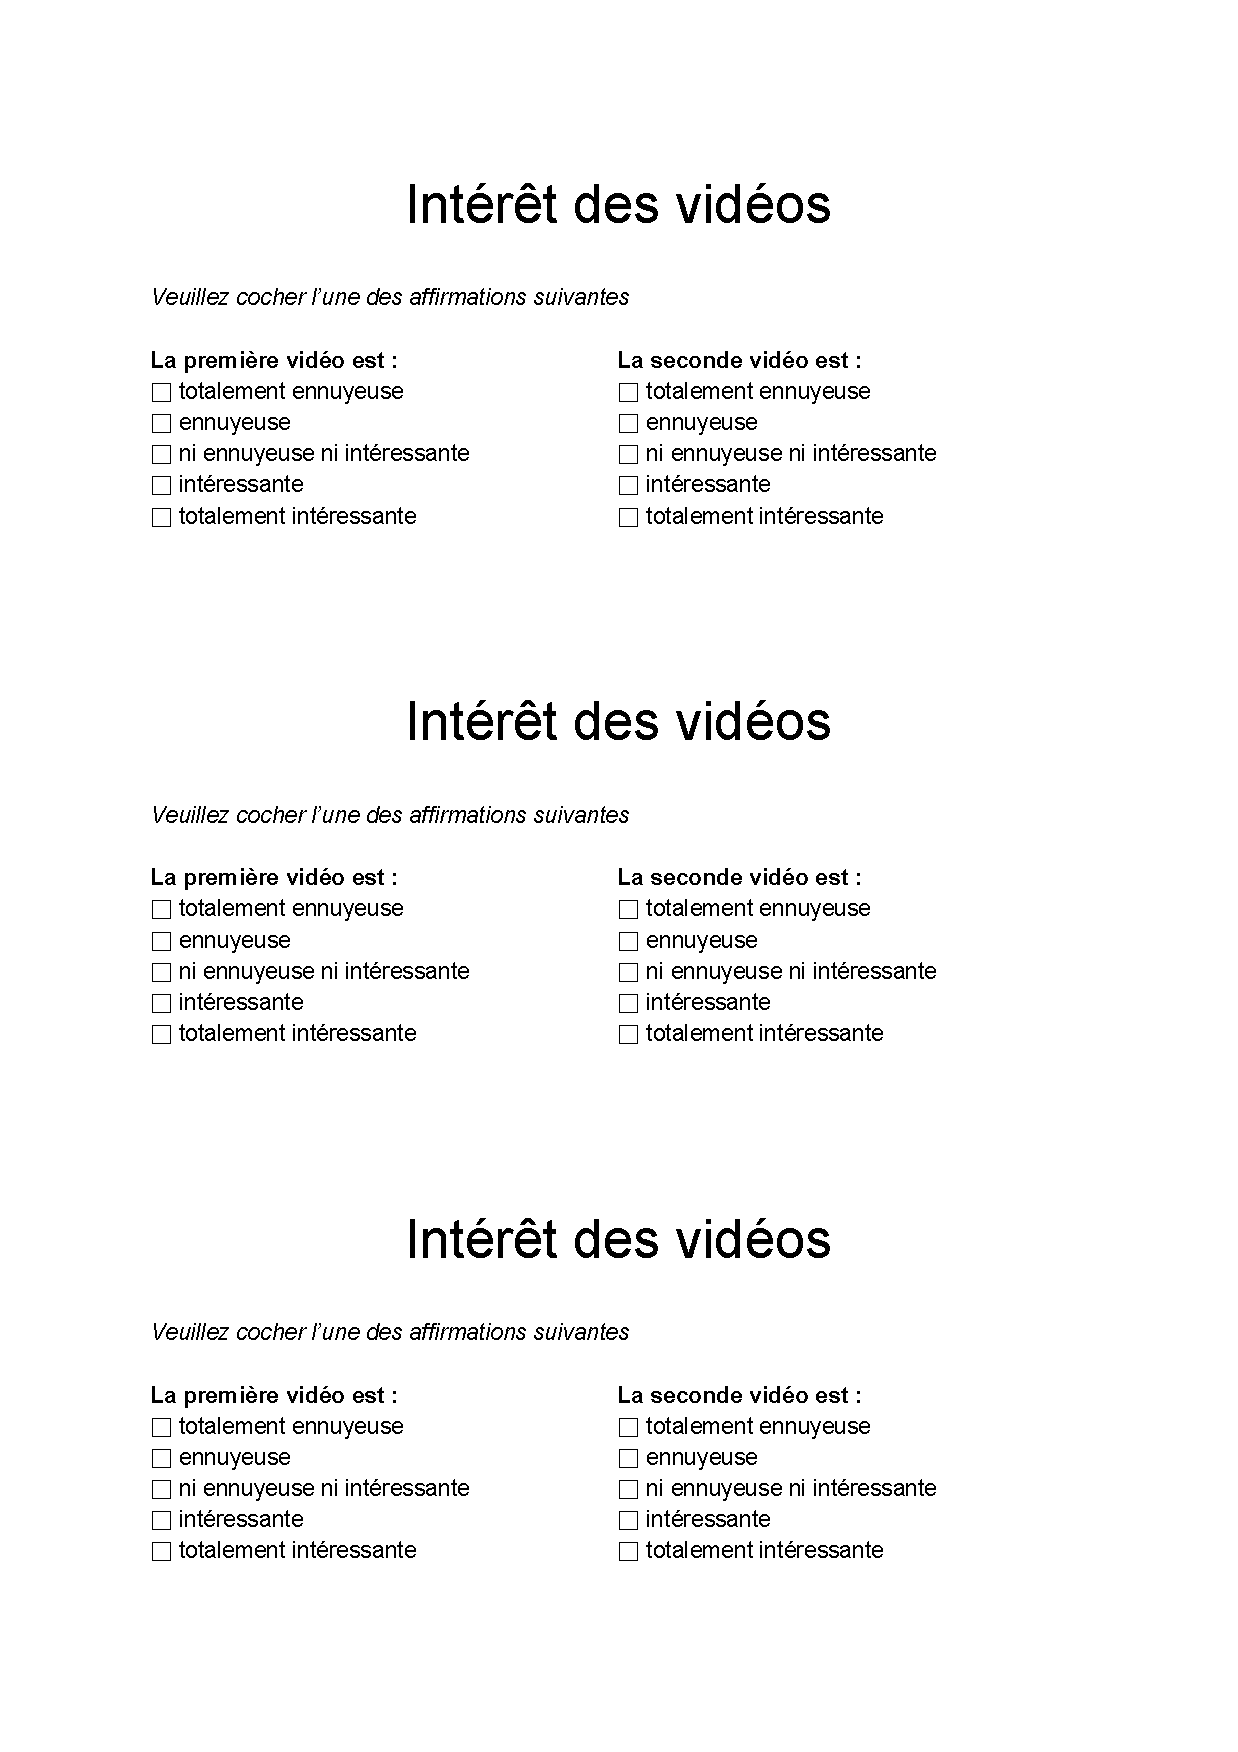
\includegraphics[trim= 40 40 40 80, clip, width=\textwidth]{exp/QuestCompl}}
	\caption{Questionnaire distribué lors de l'expérience complémentaire}
\end{figure}

\clearpage
\section*{Expérience 2}
\addcontentsline{toc}{section}{Expérience 2}
\subsection*{Chronomètre} \label{sec:chrono}
\addcontentsline{toc}{subsection}{Sudoku}
\begin{figure}[htp] \centering{
		\includegraphics[width=\textwidth]{mockup.png}}
	\caption{Interface du chronomètre utilisé lors de l'expérience 2}
\end{figure}
Le logiciel en question est disponible aux adresses suivantes :
\begin{itemize}
\item \url{http://nog5.com/files/request20.v2.exe} (serveur de l'auteur)
\item \url{https://github.com/Temporalite/TM/tree/master/exp%C3%A9rience/2/Timer.exe} (page GitHub du projet)
\end{itemize}

%----------------------------------------------------------------------------------------
%	Bibliographie
%----------------------------------------------------------------------------------------

\chapterimage{head4.jpg} % Chapter heading image

\chapter{Bibliographie}

\nocite{imgtitre,imgheader1,imgheader2,imgheader3,imgheader4,imgheader4,imgheader5,logo,analysedonnees} % Toutes les référence qui ne sont pas présentes dans le texte.

\begin{remark}
	Les illustrations de ce travail sont toutes libres de droits. Les deux vidéos utilisées appartiennent quant à elles à leurs auteurs respectifs.
\end{remark}

\section*{Livres}
\addcontentsline{toc}{section}{Livres}
\printbibliography[heading=bibempty,type=book]
\section*{Articles}
\addcontentsline{toc}{section}{Articles}
\printbibliography[heading=bibempty,type=article]
\section*{Non publié}
\addcontentsline{toc}{section}{Non publié}
\printbibliography[heading=bibempty,type=unpublished]
\section*{Ressources en ligne}
\addcontentsline{toc}{section}{Ressources en ligne}
\printbibliography[heading=bibempty,type=online]

%----------------------------------------------------------------------------------------


%EXEMPLE DE NOTEs DE BAS DE PAGE QUI PRENNENT TROP DE PLACE
% \footnote[200]{John. H. WEARDEN et Bairbre MCSHANE. «\,Interval production as an analogue of the peak procedure : Evidence for similarity of human and animal timing processes\,». In : The Quarterly Journal of Experimental Psychology Section B 40.4 (oct. 1988), pages 363–375}
% \footnote[201]{ibid}
% \footnote[202]{ibid}
% \footnote[203]{Catalin V. BUHUSI et Warren H. MECK. «\,What makes us tick ? Functional and neural mechanisms of interval timing\,». In : Nature Reviews Neuroscience 6.10 (oct. 2005), pages 755-765}
% \footnote[204]{op cit John. H. WEARDEN (1998)}
% \footnote[205]{ibid}
% \footnote[206]{Sylvie DROIT-VOLET. «\,Time perception, emotions and mood disorders\,». In : Journal of Physiology-Paris 107.4 (sept. 2013), pages 255-264}


\end{document}
